\chapter{Aspects for further standardisation activities}
In this chapterr various aspects of the subject oriented modelling and programming concept are outlined. These aspects are already published on different confernces. The following sections are based on these publications.
The concepts described in theses sections will be part of future standardisation activities.
The following sections are based on following publications:\\
\begin{list}{-}{spacing}
	\item Subjects and Shared Input Pools:
	\item Hierarchies in Communication Oriented Business Process Models:
	\item Business Activity Monitoring for S-BPM:
	\item Subject Oriented Project Management:
\end{list}

\section{Subjects and Shared Input Pools}

Shared input pools have the same structure like subject-specific ones, and thus, the same properties like the standard input pool. The only difference is that different subjects can deposit in or remove messages from a shared input pool. Subjects that want to send a message via a shared input pool do not use a subject name as addressee of a message, but the name of a shared input pool instead. In a distributed system several shared input pools for different purposes can be used. Figure 7 shows the slightly changed structure of the traffic management system when operating it with a shared input pool. The subject "Car detection" represents the shared input pool.


\begin{figure}
	\centering
	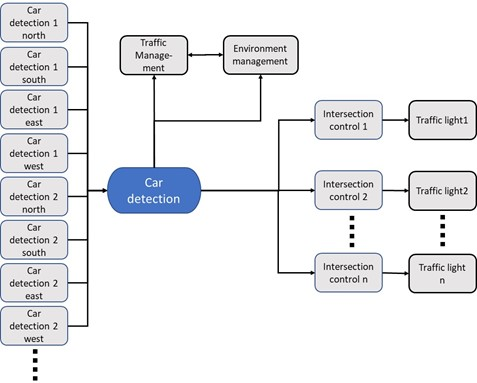
\includegraphics[width=0.7\linewidth]{Figures/Chapter5/figuresshared/SharedInputPoolExample.jpg}
	\caption[Traffic Management System with Shared Input Pool]{Traffic Management System with Shared Input Pool}
	\label{fig:SharedInputPooTraffic}
\end{figure}


Shared input pools make a distributed system more flexible when additional participants or nodes are added. For instance, a third intersection control could be added to the traffic management system without much effort. In this case, only the additional detectors and the components for controlling the intersection have to be complemented and linked to the shared input pool. The extension would have no impact on the behavior of the other subjects and their behavior in that system.
There is one additional attribute for shared input pool: It defines whether a message will be removed from the input pool once a message has been picked up by a receiving subject. This mechanism is required, since several subject may need to process a particular message. In addition, it allows keeping historical information in the input pool, in particular for analyzing the content of an input pool independently of the behavior of interacting subjects. 
The messages of an input pool can be analyzed with respect to certain patterns of its messages. In order to perform such an analysis, Complex Event Processing (CEP) concepts can be applied. Complex Event Processing can be encapsulated in a subject. A subject of this kind scans the messages of a shared input pool and checks whether patterns of interest can be found. Once such a pattern is identified, a message including the discovered pattern can be sent to other participants, and initiate further activities. Figure 8 shows the traffic management example enriched with subjects processing complex events.
In the example, the subject "CEP pollution analyzer" can analyze the time between cars passing the intersection in a certain time period. It can identify the events "low traffic" or "high traffic" and send it to the subject "Environment management". In case of tunnels, the subject "Environment management" might react to this information in a different way compared to open air settings. 


\begin{figure}
	\centering
	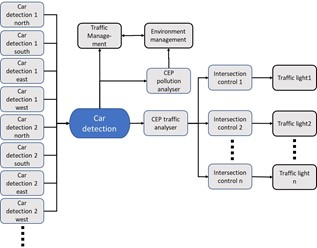
\includegraphics[width=0.7\linewidth]{Figures/Chapter5/figuresshared/SharedInputPoolEvent.jpg}
	\caption[Shared Input Pools and Complex Event Processing]{Shared Input Pools and Complex Event Processing}
	\label{fig:sharedInputPoolEvents}
\end{figure}

\subsection{Implementing Shared Input Pools}
As mentioned earlier, shared data repositories represent a single point of failure of a distributed system. A malfunction of a shared data storage component or device may have a significant impact on the functionality of the whole distributed system. If a subject or a communication line is disturbed, only a small part of a system may be concerned but if a shared data store is down this has an impact on all subjects accessing this input pool.
\\
In addition to this operational problem it must be decided in the course of organizational implementation which organization is held responsible for running and maintaining the system hosting the shared data. Such issues become prominent, if a distributed system is connecting several independent organizations, e.g., different companies in a supply chain. Distributed systems run by independent organizations may also have to deal with several changes dynamically, affecting the data quality and system stability. Even companies can be replaced by other organizations. If only functional subjects are concerned, such a change can be managed without affecting the operation of the entire system: The execution of a subject is just assigned to the new actor. The problem is more serious if a company leaving a distributed system is responsible for running the system with shared data, as other participants of the shared system are affected. Then, a new company still part of the distributed system must take over the responsibility for the shared data. The migration of these data from one company to another can become very cumbersome from the business point of view and from a technological perspective, too.
One way to solve these problems is implementing shared input pools with blockchain technology. A blockchain is an open, distributed ledger that can record transactions efficiently in a verifiable and permanent way. Blockchains allow to achieve the integrity of a collection of data in a distributed peer-to-peer system, whereas the number of the peers is unknown and an unknown number of them are not reliable and trustworthy \cite{book:Blockchainbasics}. 
\\
Today, blockchains are mainly used for managing the ownership of money, goods, real estates, etc. Each participant in a distributed system may have a copy of a blockchain. Changes in a blockchain follow a mechanism which manage changes in a consistent way and the change protocol guarantees that any participant will have again a consistent copy after a change. A change of a blockchain means that a new data record is added, and nothing can be removed from a block chain. Adding a new block to a block chain requires some effort from parties involved in a blockchain. This effort is rewarded by adding crypto money to the party when having accomplished the task successfully. These rewards serve as an incentive for the creators of blocks. 
\\
Although heavily questioned with respect to effort and gains by practitioners \cite{article:BlockchainUniverse} blockchain technology provides concepts ensuring the trustworthiness of system components. The latter becomes crucial when operating sensitive distributed systems, such as public transportation and healthcare, in particular when event-based data fusion is needed, where nodes of various type (sensor systems, vendor-specific monitoring systems. user devices, household items, etc.) exchange notifications of events and decision-relevant data with each other. In such settings, not only notification mechanisms needs to be streamlined in case of heterogeneity of nodes, but also data source trust is important for further processing and system behavior \cite{article:EventbasedSensor}.
\\ 
In order to ensure dependable sharing of data, these basic properties of blockchains need to be adapted to the requirements of a shared input pool. Hence, a blockchain-oriented implementation of a shared input pool must meet several requirements:
\begin{enumerate}
	\item Subjects can subscribe for the access to a shared input pool.
	\item Subjects subscribed for an input pool may deposit or read events from that input pool. 
	\item Events can be marked as removed from a shared input pool.
	\item Subjects may analyze the content of a blockchain, e.g., when processing complex events.
	\item There must be a mechanism that a block chain can be deleted, once all involved parties agree on that.
\end{enumerate}

Traditionally data received from "things" are not very complex. These data are mainly values as measured by sensors, or binary signals. This may lead to a paradox situation: If such simple data are to be stored in a blockchain, the fee to be paid for adding blocks containing simple data is larger than the value being transferred. 
One way to solve the resulting incentive problem is to use permissioned block chains instead of open block chains: Blockchain for dedicated distributed application are not open blockchains like the ones implementing the management of digital currencies. 
\\
For the implementation of shared input pools, we suggest managed or permissioned blockchains. For instance, Hyperledger Fabric \cite{article:hyperledger} is an open source implementation of a permissioned blockchain. Unlike to a public permissionless network, the participants are known to each other, rather than staying anonymous and interacting untrusted. It means, while the participants may not fully trust one another, e.g., in case of being competitors in the same industry sector, a network can be operated under a governance model that is built on the extent of trust existing between participants, such as a legal agreement or framework for handling disputes. When building a business process with known participants, such type of a blockchain implementation would be sufficient. Consensus algorithms for permissioned blockchains are faster and do need much less energy than permissionless blockchain networks. 
\\
In \cite{article:Blockbench} it is reported that hyperledger fabric is the fastest available permissioned blockchain. The transaction throughput could even increased from 3,000 to 20,000 transactions per second \cite{article:hyperledgerfabric}.
\\
When using Hyperledger to create blockchain networks of that kind, a hyperledger blockchain network provides a technical infrastructure offering ledger and smart contract (chaincode) services to applications. Primarily, smart contracts are used to generate transactions which are subsequently distributed to every peer node in the network where they are immutably recorded on their copy of the ledger. The users of applications can be users of client applications or blockchain network administrators.
\\
Subject add messages to the shared input pool and other subjects want to read these messages. If a shared input pool is implemented as a blockchain it is necessary that the chain code (smart contract in Ethereum) realizing the functions of the shared input pool must interact with the world outside the block chain. In hyper ledger fabric (including Ethereum), this problem is solved by so called oracles. We suggest using the blockchain patterns Oracle and Reverse Oracle as described in \cite{book:Blockchainapplications}. For flexibility reasons we prefer off chain oracles - see figure \ref{fig:sharedblockchain}.



\begin{figure}
	\centering
	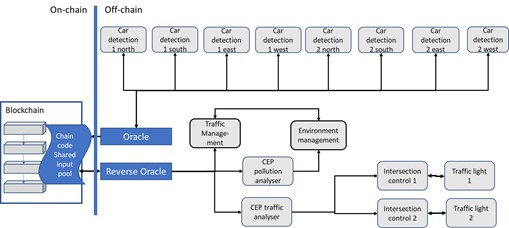
\includegraphics[width=0.7\linewidth]{Figures/Chapter5/figuresshared/Block-Chain.jpg}
	\caption[Utilizing block chain patterns Oracle and Reverse Oracle]{Utilizing block chain patterns Oracle and Reverse Oracle}
	\label{fig:sharedblockchain}
\end{figure}


\section{Hierarchies in Communication Oriented Business Process Models}
PASS  offers powerful possibilities for structuring complex process systems. The ways to do that are demonstrated with an example.
As an example we will consider a process for realizing a car break down service. This service con-sists of several connected processes. There is the main process for handling the car accident and supporting e.g. processes for organising towing and repair shop services. Insurance companies may be involved for covering damages, the customer gets an invoice, uses money transfer services or banks for paying the invoice. These processes are executed by various organisations like help desk service companies, towing service companies, car repair workshops banks etc.. In most business process projects not complete processes are described in detail only a certain part is considered e.g. only the help desk process has to be considered in detail but to do that we have to considere the whole environment in which a considered process is embedded. We have to know which rela-tions exists to these other processes. It is necessary to know which inputs are rquired by neighbour processes and which results they deliver. A help desk process which organizes the towing services has to know how the towing service is requested and which further interactions are required. For instance it must be agreed whether the towing service informs the client about the arrival time of the towing truck or the help desk does it.


\subsection{Process Architecture}

Rectangles represent processes. Each process has a name. Processes consists of other processes and/or subjects. The lines between the rectangles represent the communication channels between processes. Each communication channel has a nameand can contain other communication chan-nels and/or messages.

Figure \ref{fig:car-service-level1} shows the highest process level of the car break down service. In the "car use" process the event "car break down" happens. In order to organize support an interaction is initiated with process "car break down service" . Between these processes messages are exchanged which are elements of the communication channel "Car break down handling".\\


\begin{figure}[ph]
	\centering
	
\includegraphics[width=0.7\linewidth]{Figures/Chapter5/figures-hierarchy/Car-Service-Level1.jpg}
	\caption[High level structure of car break down service]{High level structure of car break down service}
	\label{fig:car-service-level1}
\end{figure}



Figure \ref{fig:car-service-leve2} shows the next process structure level of the process "car break down ser-vice". In this level the process "Car break down service" is separated in 10 processes. The processes "Bank", "Insurance service", "Car repair workshop", "Incident Management","Mobility Manage-ment" and "Towing Management" have a communication channel to the prcess "Car usage". This means the communication channel "Car break down handling" is separated into five communica-tion channels. Each of them covers the communication with the relared process, e.g. the communi-cation channel "Accident notification Car break down" is the communication channel between the processes "Car usage" and "Incident Management".\\


\begin{figure*}
	\centering
	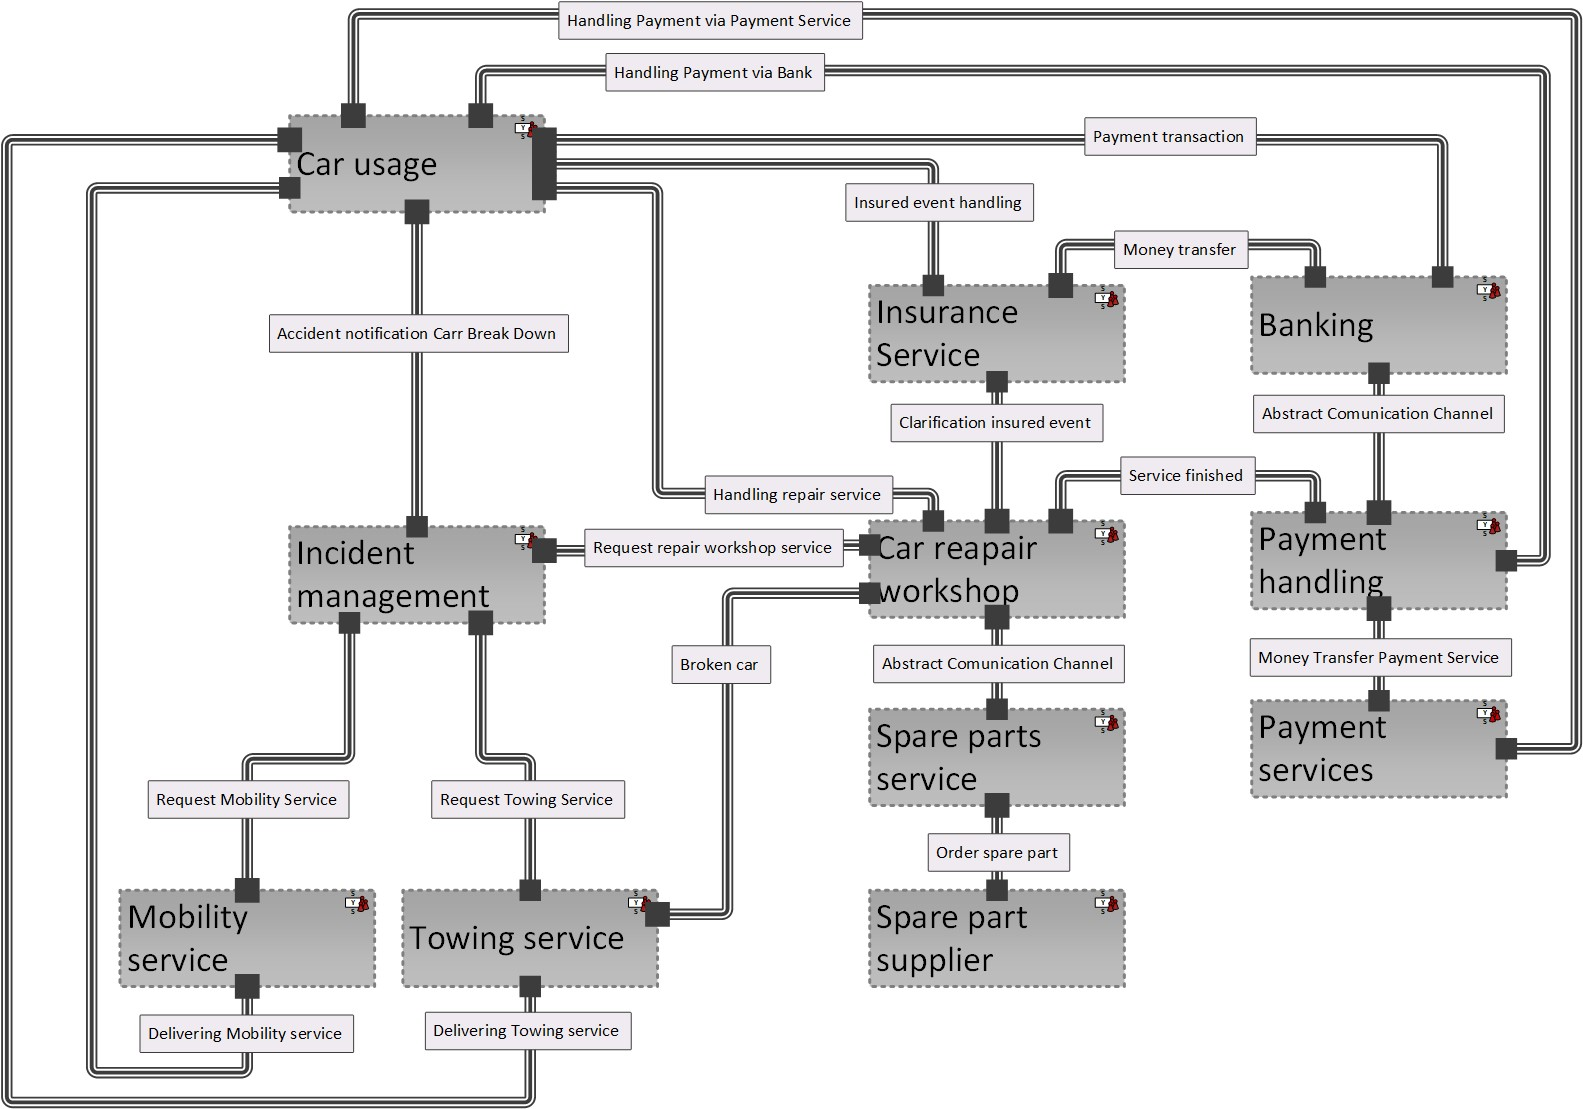
\includegraphics[width=0.8\linewidth]{Figures/Chapter5/figures-hierarchy/Car-Service-Leve2}
	\caption[Structure of the Emmergency Call Handling Process]{Structure of the Emmergency Call Handling Process}
	\label{fig:car-service-leve2}
\end{figure*}



Inside a process there can be also processes. This means that levels of processes can be built. Figure \ref{fig:car-service-lev3} shows the next deeper level of our process hierarchy. The process "Car repair workshop" is structured in six processes. According to this separation the communication sets are also splitted e.g. the communication set "Handling repair service" is splitted into three parts, one part is han-dled by the process "Service scheduling" the other by the process "Car droping" and the third one by the process "Customer Satisfaction".\\

\begin{figure*}
	\centering
	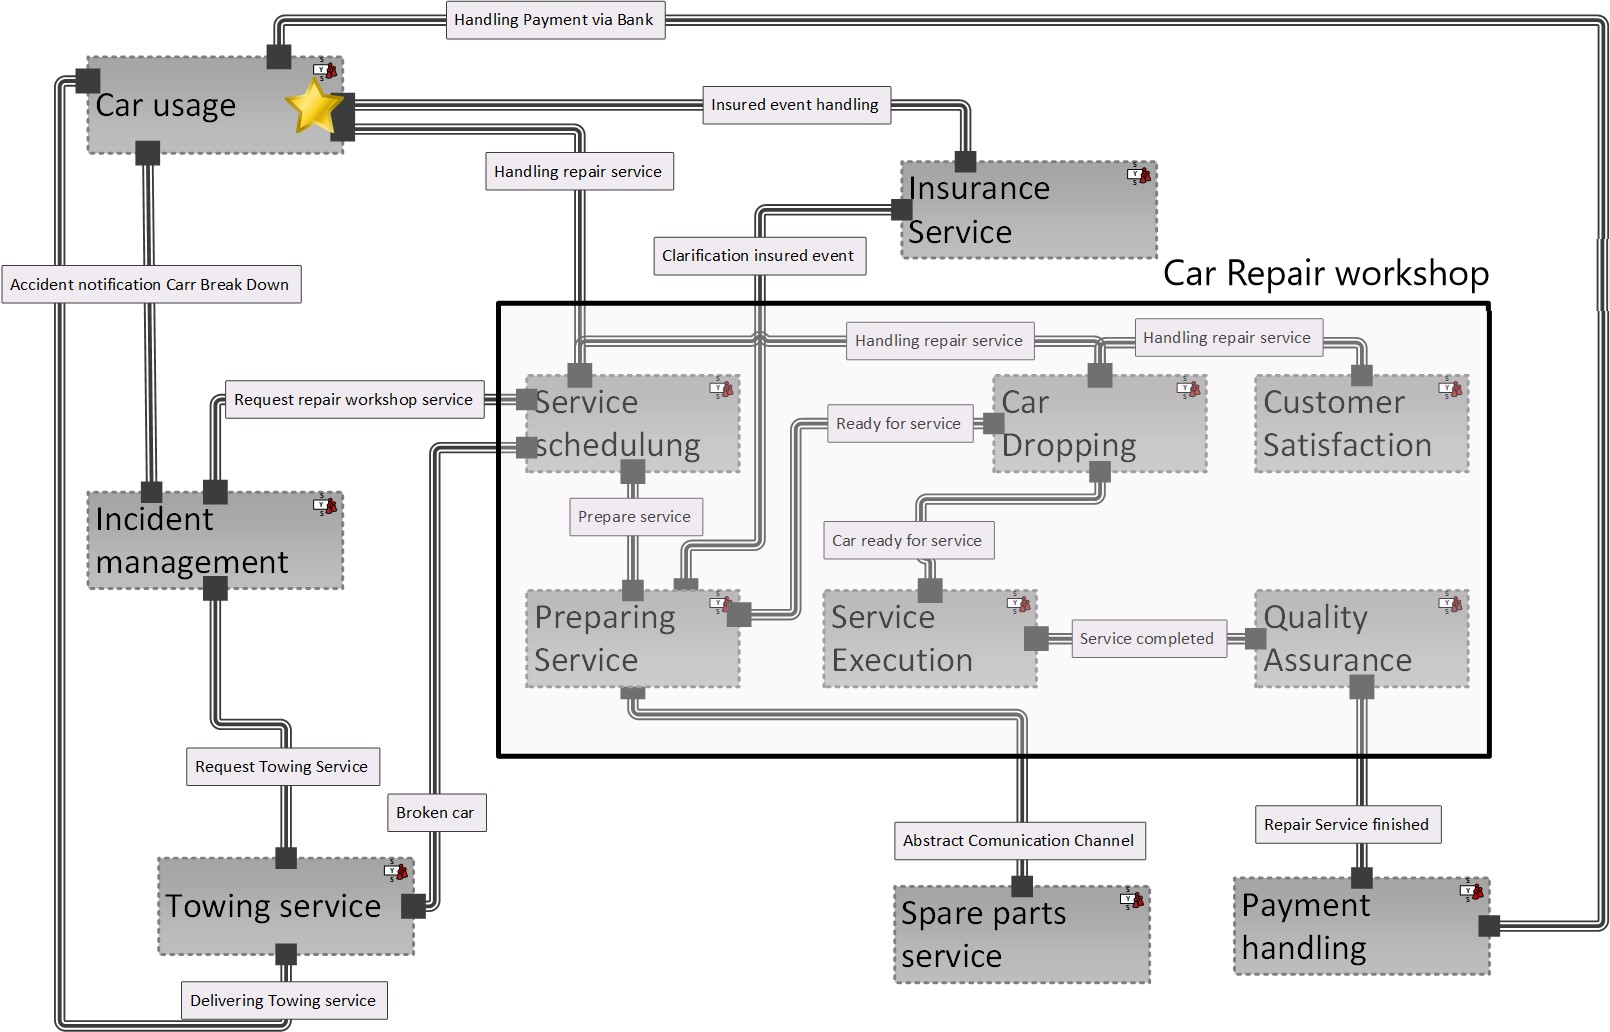
\includegraphics[width=0.8\linewidth]{Figures/Chapter5/figures-hierarchy/Car-Service-Lev3}
	\caption[Details of the "Car repair workshop" Process]{Details of the "Car repair workshop" Process}
	\label{fig:car-service-lev3}
\end{figure*}

As already mentioned, processes cannot communicate directly with each other. The active entities of a process, the subjects communicate with each other. This means messages from one process are sent to an other process are reveived by a subject inside of that process. Messages belonging to a channel are assigned to a sending or receiving subject at the lowest level of an process architecture. This lowest level of a process description is the subject interaction diagram (SID) which shows the involved subjects of a process and the messages they exchange. In the following we consider the process incident management in more detail. This process does not contain other processes like the process "Car Repair Shop". The process "Incident management" contains a Subject Interaction Diagram. Some of the subjects of a process communicate with subjects in other processes. These subjects are called border subjects because they are at the border of a process to other prcesses. Figure \ref{fig:car-service-lev4} shows the process "Incident management" with its border subjects. There is a border subject "Help agent" which communicates with the processes "Towing service", "Mobility ser-vice"and  "Car repair workshop", precisely it communicates with a subject in one of these process-es. Another border subject of the process "Incident management" which is called "Help desk"communicates with the process "Car usage".\\

\begin{figure}[ph]
	\centering
	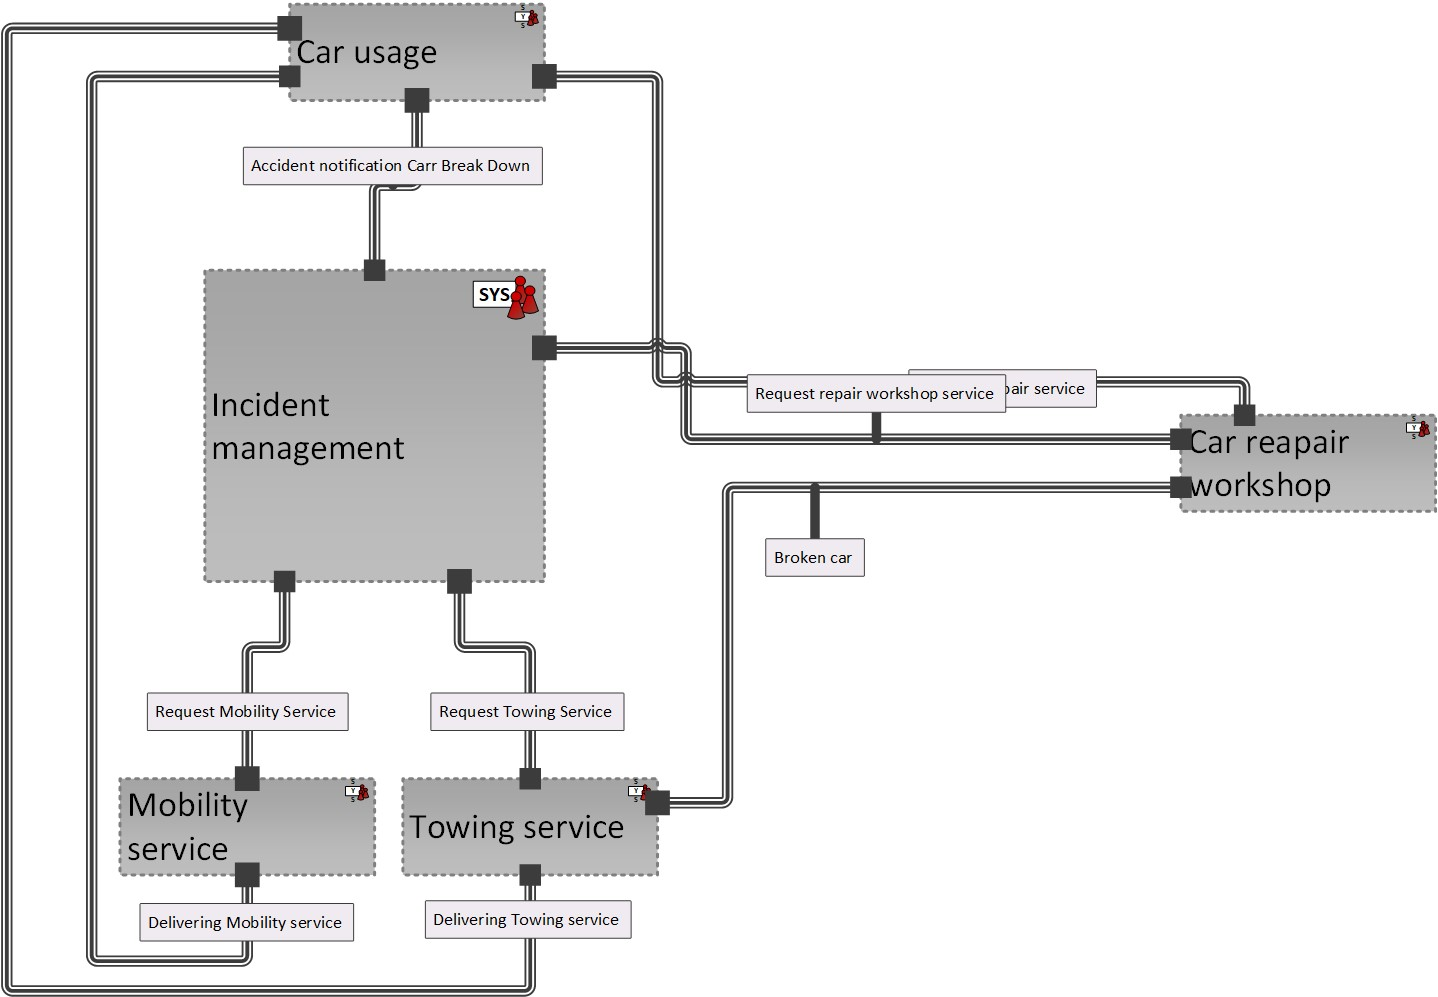
\includegraphics[width=0.9\linewidth]{Figures/Chapter5/figures-hierarchy/Car-Service-Lev4}
	\caption[Neighbors of the "Incident Manaement Process"]{Neighbors of the "Incident Manaement Process"}
	\label{fig:car-service-lev4}
\end{figure}

The border subjects of the process "Incident management" must have a coresponding border sub-ject at the neighbour processes. The border subjects "Call agent" communicates with the border subject "Help requestor" of process "Car usage" and the border subject "Help agent" communi-cates with border subjects of the processes "Car repair workshop", "Towing service and "Mobility service". The process "Incident management" with all the border subjects is shown in  figure \ref{fig:car-service-lev5}.\\

\begin{figure}
	\centering
	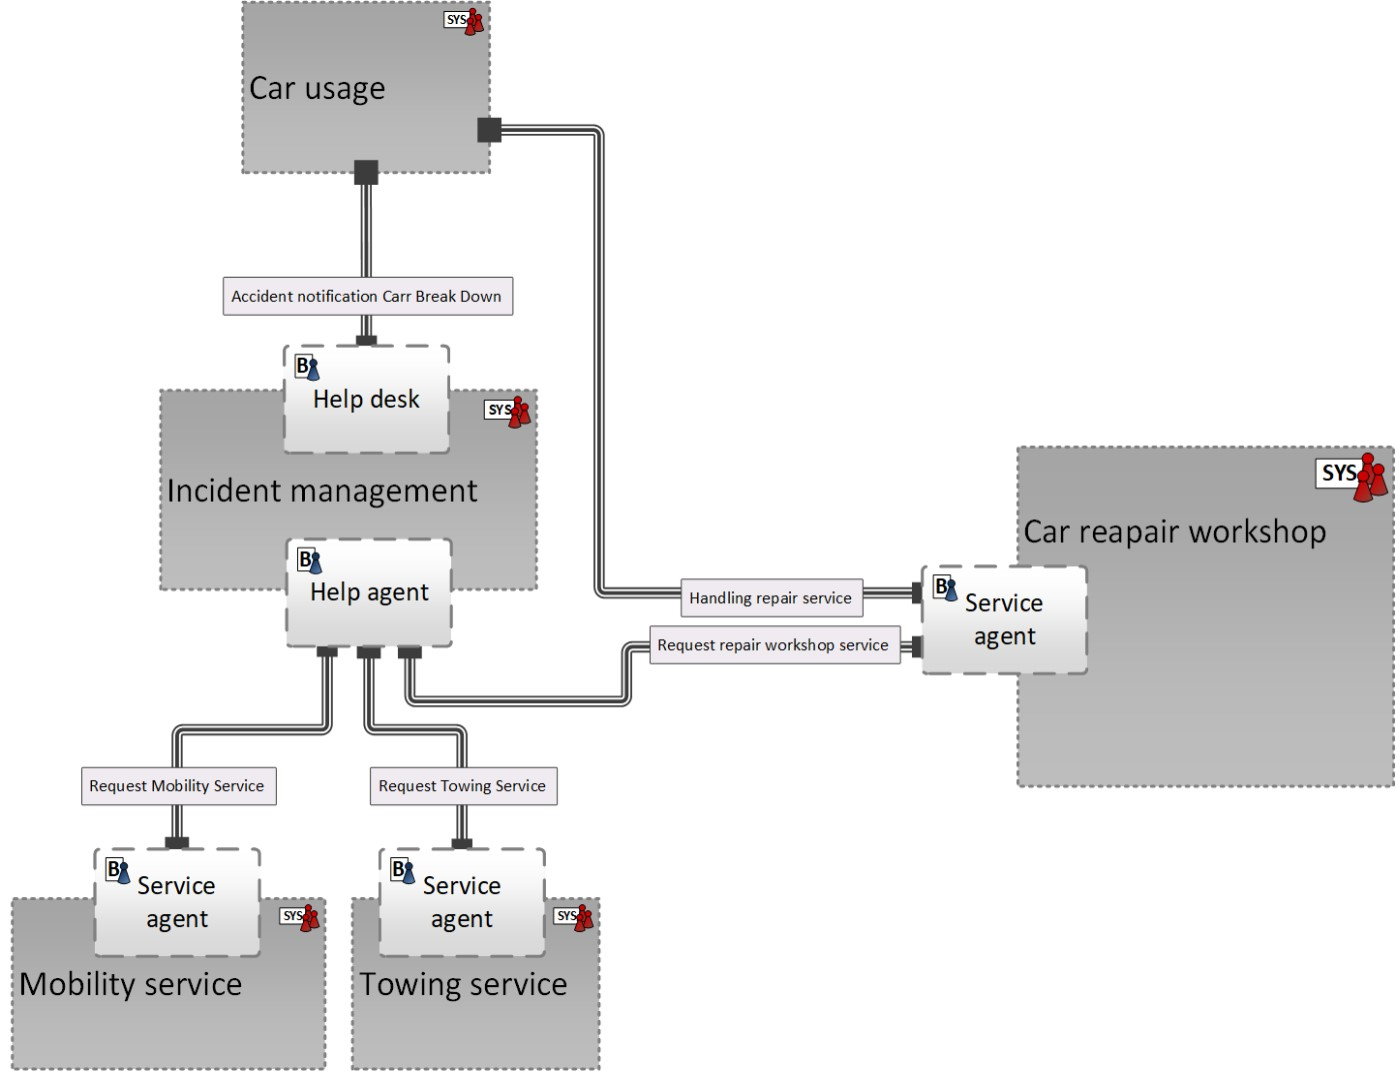
\includegraphics[width=0.9\linewidth]{Figures/Chapter5/figures-hierarchy/Car-Service-Lev5}
	\caption[Border subjects of the "Incident Management" Process]{Border subjects of the "Incident Management" Process}
	\label{fig:car-service-lev5}
\end{figure}

The border subjects of the processes "Mobility service", "Towing service" and "Car repair work-shop" have the same name “Service agent” but these are different subjets because they belong to different processes. Because the process "Car repair workshop" consists of several layers the corre-sponding border subject can be in a process which is part of process "Car repair workshop" in a lower level.\\
From the perspective of the subjects inside of the process "Incident managent" are the border subjects of the processes "Mobility service", "Towing service" and "Car repair workshop" interfaces to these processes, therefore they are called interface subjects in the subject interaction diegram of a process. Figure \ref{fig:car-service-lev6}shows the subject interaction diagram of the process incident management.\\


\subsection{Behavioral Interface}
Processes to which a considered process has communication relationships are called process neighbours or for short neighbours. Now we want to consider the details of the communication relationships between two neighbours. The interface between two processes is defined by the related border subjects and the allowed sequences in which the messages a communication channel are exchanged between them. As already described above each message is defined by a name and the data which are transported the so-called payload. A border subject observes the behavior of the border subject of the neighbour process and vice versa. Figure \ref{fig:car-service-lev8} shows the border subject "Help desk" of the processes "Incident Management" which communicates with the border subject of process "Car usage".\\

\begin{figure}
	\centering
	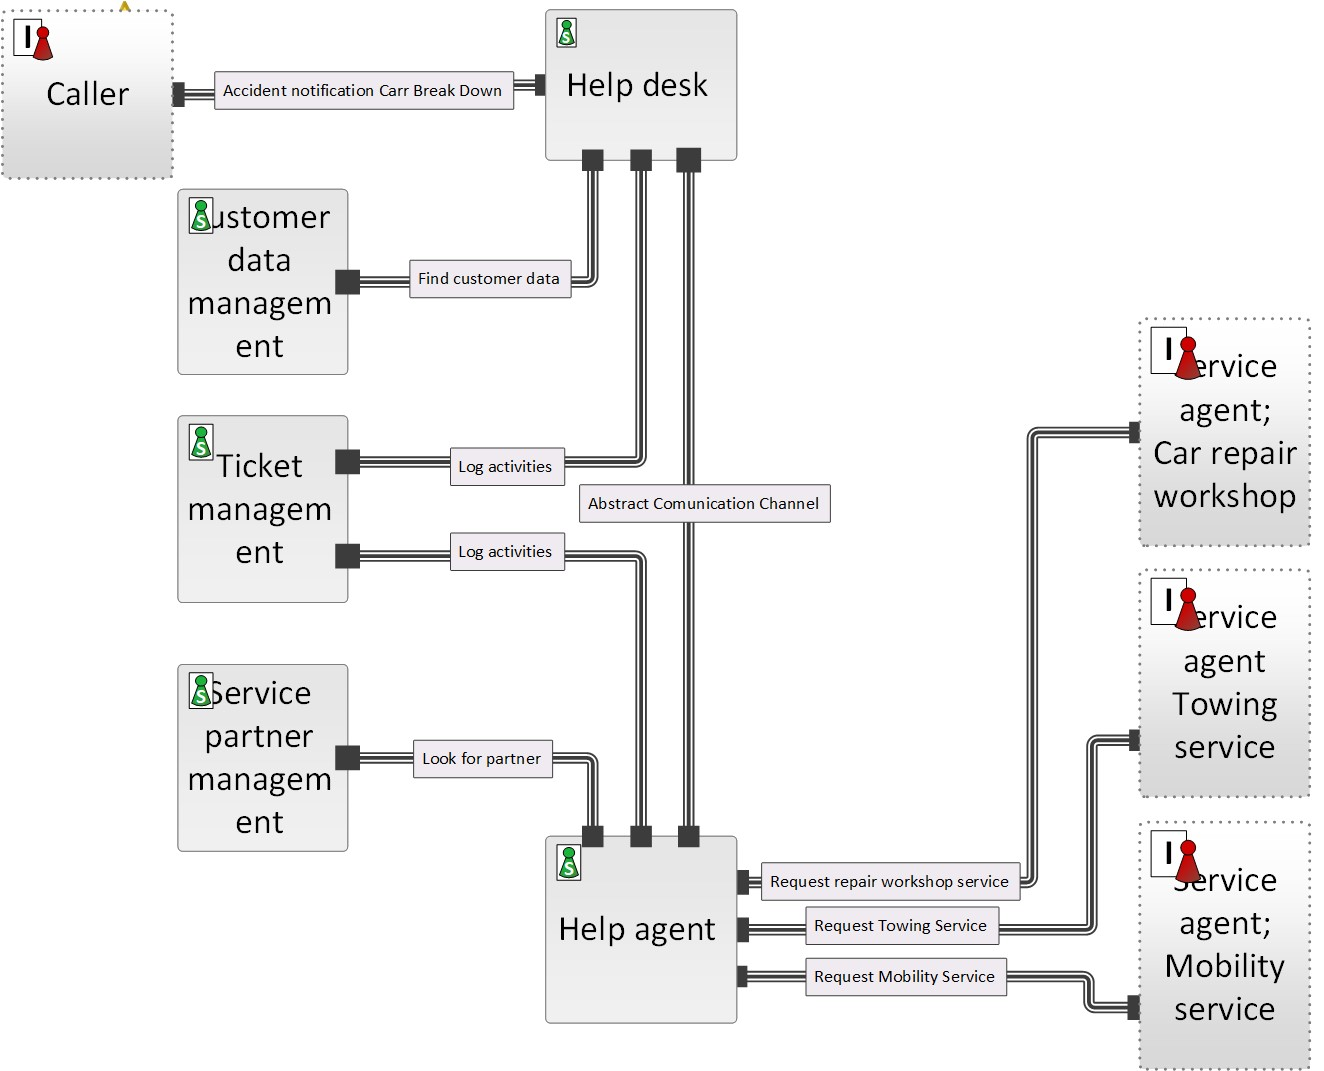
\includegraphics[width=1.0\linewidth]{Figures/Chapter5/figures-hierarchy/Car-Service-Lev6}
	\caption[Subject Interaction Diagram of the Process "Incident Management"]{Subject Interaction Diagram of the Process "Incident Management"}
	\label{fig:car-service-lev6}
\end{figure}

Because we consider the process "Incident management" the border subject "Caller" of the process "Car usage" becomes an interface subject in the SID (details about interface subjects can be found in \cite{Flei12}) of the process “Incident Management”. Figure \ref{fig:car-service-lev8} shows the detailed subject interaction diagram around the subject help desk. \\

\begin{figure}
	\centering
	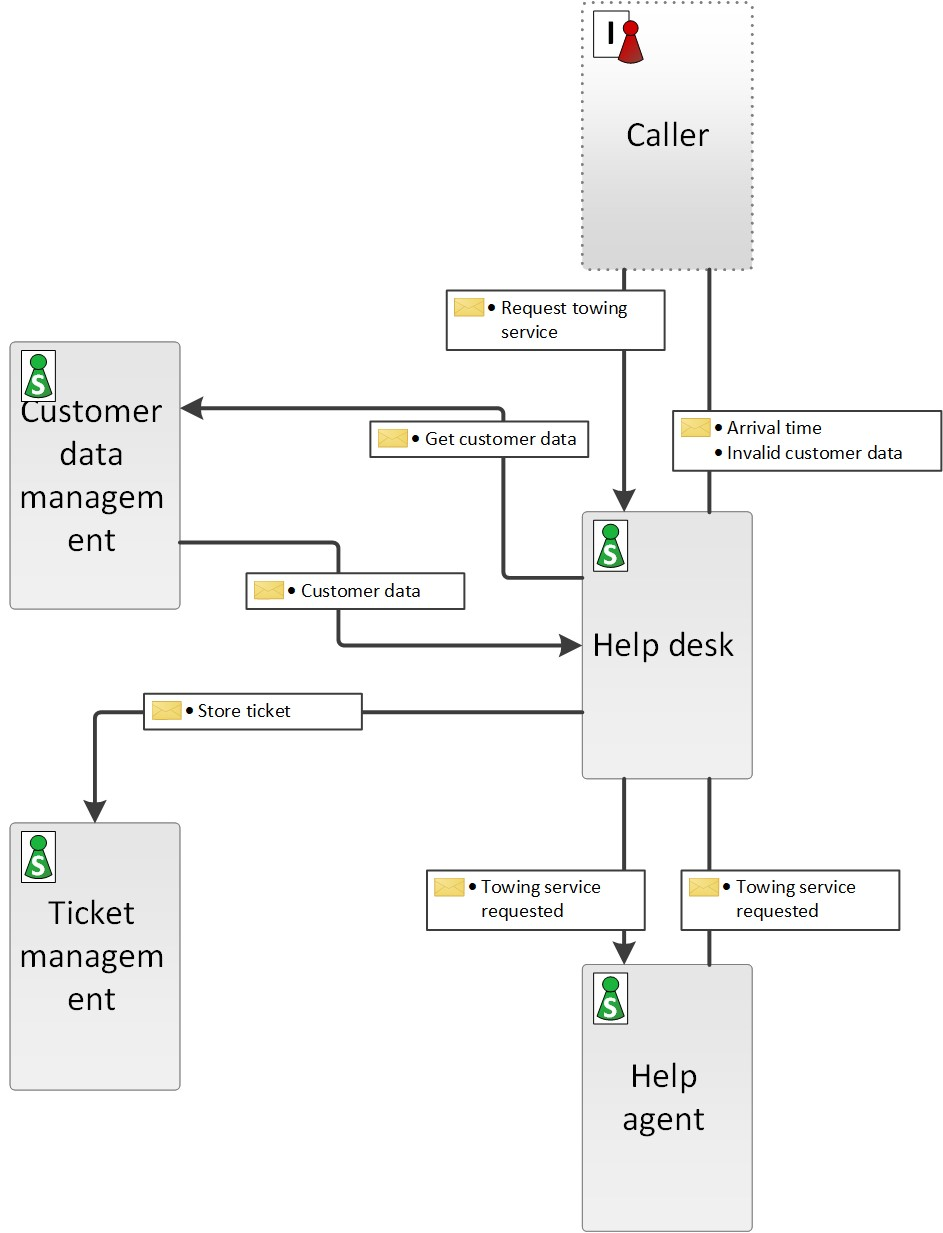
\includegraphics[width=0.9\linewidth]{Figures/Chapter5/figures-hierarchy/Car-Service-Lev8}
	\caption[Subject Interaction around the subject “Help desk”]{Subject Interaction around the subject “Help desk”}
	\label{fig:car-service-lev8}
\end{figure}

Instead of the channels the messages required for a towing service request are shown. A message "Request towing service" comes from the interface subject. This message is accepted by the subject "help desk". The subject help desk checks the customer data received with this message by sending a corresponding the message "Get customer data" to the subject "Customer data management". This subject send the complete customer data back to the subject "Help desk" via the message "Customer data". The subject "Help desk" checks the customer data. If the data are invalid a message "Invalid customer data" is sent to the subject "Caller" and the process is finished.\ 
If the customer data are valid with that data the subject "Help desk" creates a trouble ticket which is sent to the subject "Ticket management". After that the message "Towing service requested" is sent to the help agent which organizes the towing service. The part of the communication structure of the subject "Help agent" in order to organize the towing service is not shown in figure \ref{fig:car-service-lev9}. We only see that subject "Help agent" sends the message "Towing service data" to the subject "Help desk". This message contains all the data about the service e.g. name of the towing company and arrival time. The subject "Help desk" forwards that data to the interface subject "Caller". This behavior is shown in figure \ref{fig:car-service-lev8}.\\



\begin{figure}
	\centering
	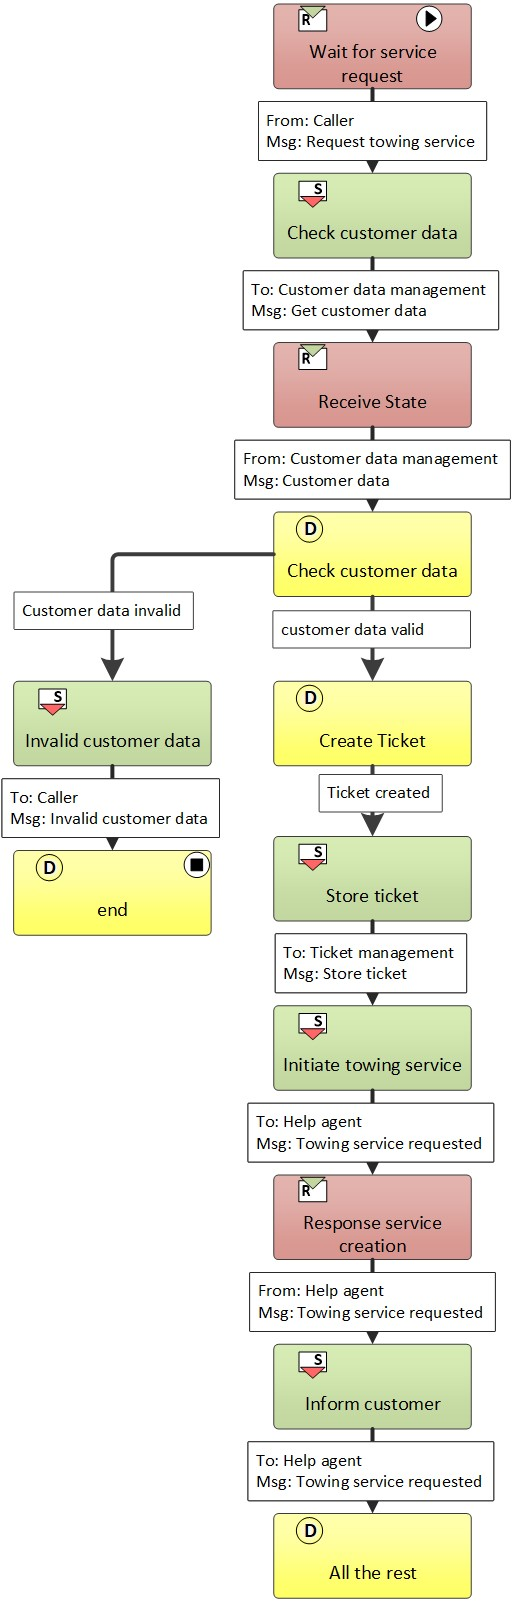
\includegraphics[width=0.7\linewidth]{Figures/Chapter5/figures-hierarchy/Car-Service-Lev9}
	\caption[Part of the Behavior Diagramm of the subject “Help desk”]{Part of the Behavior Diagramm of the subject “Help desk”}
	\label{fig:car-service-lev9}
\end{figure}


The behavior described in the figure above contains the communication with all neighbor subjects of subject "Help desk" including the communication with the interface sub-ject "Caller". From the perspective of this subject the communication of the subject "Help desk" with its other neighbor subjects is not relevant. For the subject "Caller" only the commumication sequence between itself and the subject "Help desk" is relevant. These allowed communication sequences are called the behavioral interface.\\
The behavioral interface between two subjects can be derived from the complete behavior of a subject by deleting the interactions with all the other subjects . Figure \ref{fig:car-service-lev10} shows how the communication sequence relevant for the communication be-tween the subject "Help Desk" and "Caller" is derived from the complete behavior of subject "Help desk".

\begin{figure}
	\centering
	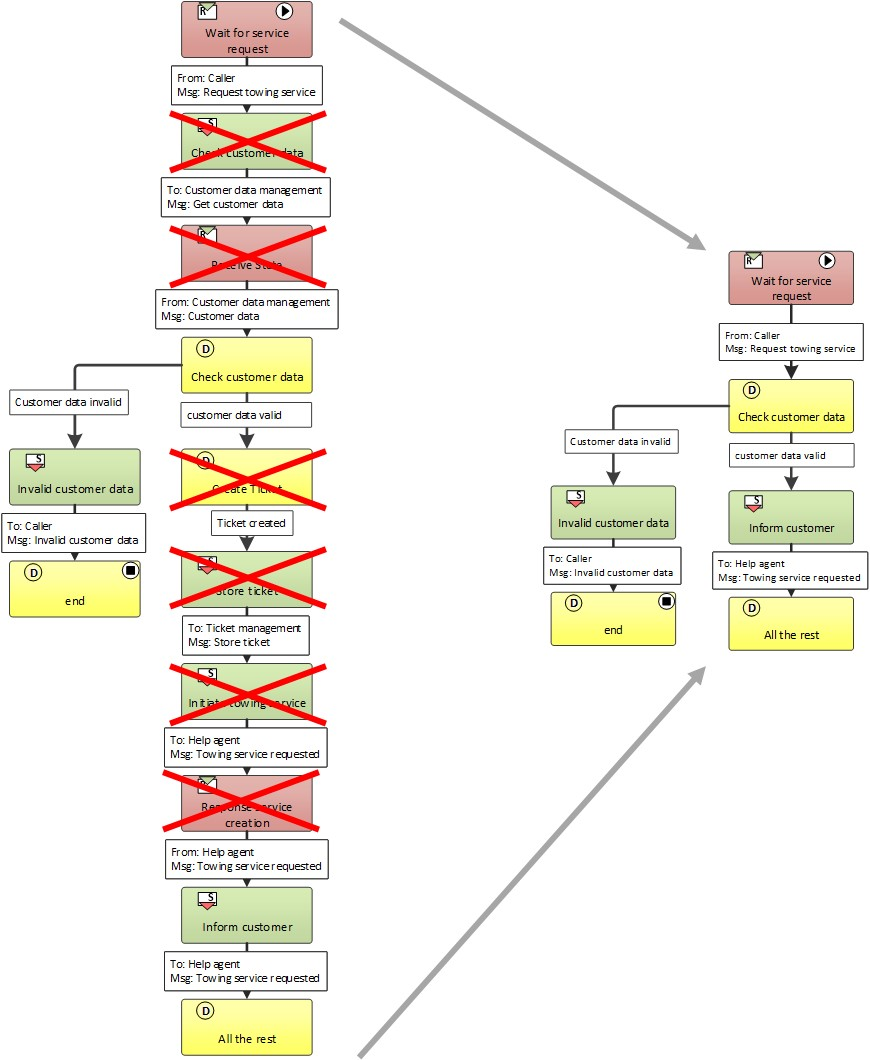
\includegraphics[width=1.0\linewidth]{Figures/Chapter5/figures-hierarchy/Car-Service-Lev10}
	\caption[Deriving the Behavioral Interface from the Subject Behavior]{Deriving the Behavioral Interface from the Subject Behavior}
	\label{fig:car-service-lev10}
\end{figure}

A behavoral interface is always relative to a communication partner. In figure \ref{fig:car-service-lev10} the behavioral interface is relative to the interface subject "Caller". The behavioral interface to the subject "Ticket Management" is different because only the communication activities with this subject are considered.This behavioral interface would be very simple. It consists of only one send activity, sending the message "Store ticket".\\
The behavioral interface relative to a partner subject can be automatically derived from the complete behavior of a subject
(see \cite{article:jCPEX}).


\section{Business Activity Monitoring for S-BPM}

Monitoring of Business Process looks at running instances. For those it measures metrics, aggregates them to Process Performance Indicators (PPIs) as a business process-related form of Key Performance Indicators (KPIs), reveals deviations (as-is vs. to-be) and report and presents results to people in charge or interested in the value of the PPI. Thus monitoring lays ground for the performance analysis in the key dimensions quality, time and costs of processes and helps identifying weaknesses and opportunities for improvement \cite{book:UntPerform}.
By feeding back information for completed and running instances to analysis monitoring fosters organizational learning, forms an important part of the Business Process Management (BPM) lifecycle \cite{article:SUbjetorientiertBPM} and thus helps implementing the operational level in the closed-loop approach to enterprise performance management \cite{book:processmonitoring} (see figure \ref{fig:Approach-Performance}).
\\


\begin{figure}[h]
	\centering
	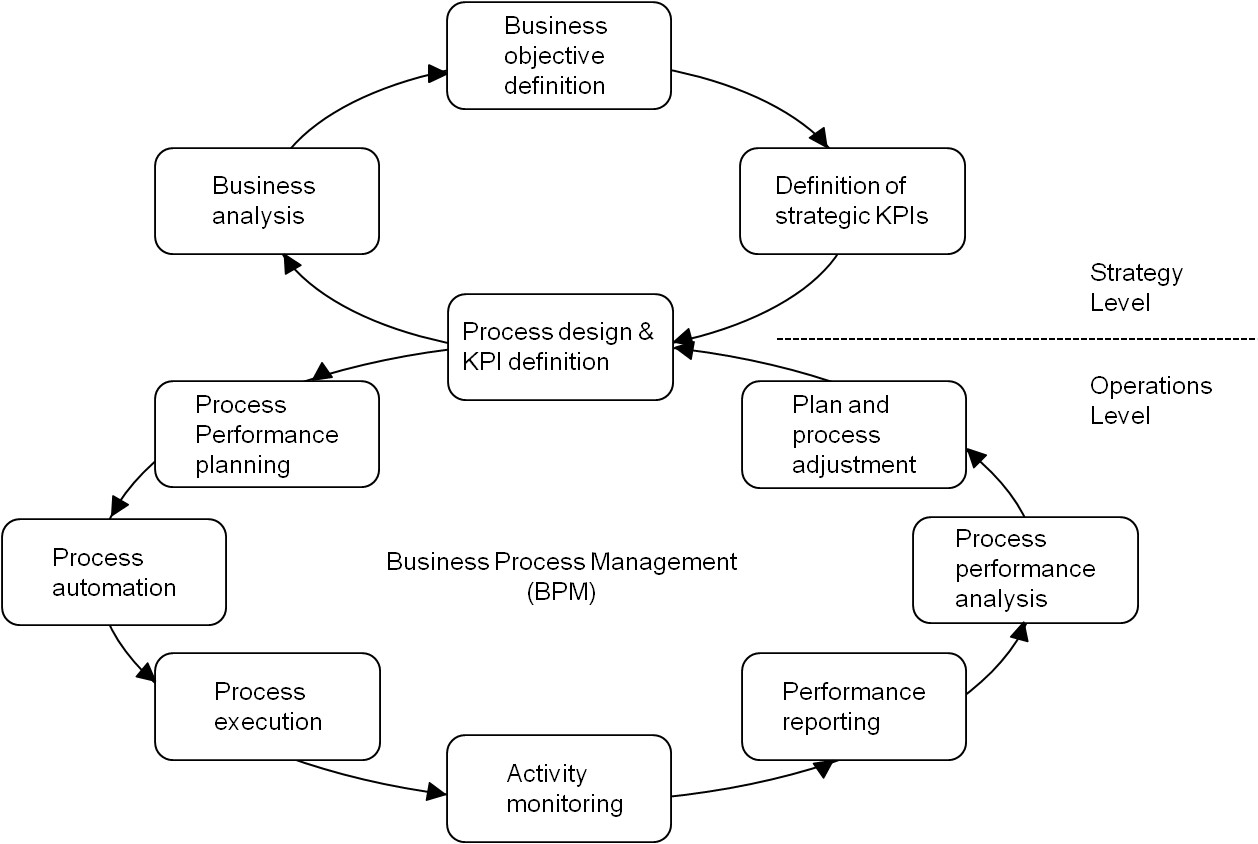
\includegraphics[width=0.8\linewidth]{Figures/Chapter5/Monitoring/Approach-Performance-Mgmt.jpg}
	\caption[Closed-loop Approach to Performance Management]{Closed-loop Approach to Performance Management \cite{book:AnalytInfSys}}
	\label{fig:Approach-Performance}
\end{figure}



\subsection{Architecture }  
A Business Activity Monitoring (BAM) environment supported by Complex Event Processing consists of several elements necessary at build time and at runtime (see figure \ref{fig:BAMArchitecture}) and \cite{book:processmonitoring}, \cite{book:CEPinAction} , \cite{article:BlueprintEventBPM}). At build time a modeling environment should provide tools for designing processes (e.g. Metasonic Build) and defining process performance indicators (PPIs), BAM events, rules, thresholds etc. as well as parameters for their visualization in report and on dashboards. At runtime there are (1) event producers like a process engine (e.g. Metasonic Flow) or an ERP system (e.g. SAP) which feed events into an event cloud or stream (chronologically ordered). (2) Event Processing Agents (EPA) form the event processing logic. They process events based on metrics, event patterns, rules and other parameters specified at design time. Their basic logical functions include filtering and transforming events and detecting patterns among them. Global state elements allow them accessing data from outside the application (e.g. from an ERP system). EPAs put the results of their processing (also to be understood as events) out to Event Consumers (3) like dashboards or process engines. Input and Output Adapters (IA, OA) transform event data between different formats of system elements as necessary. All system elements involved form an Event Processing Network (EPN), in which events are exchanged by communication mechanisms.

\begin{figure}[h]
	\centering
	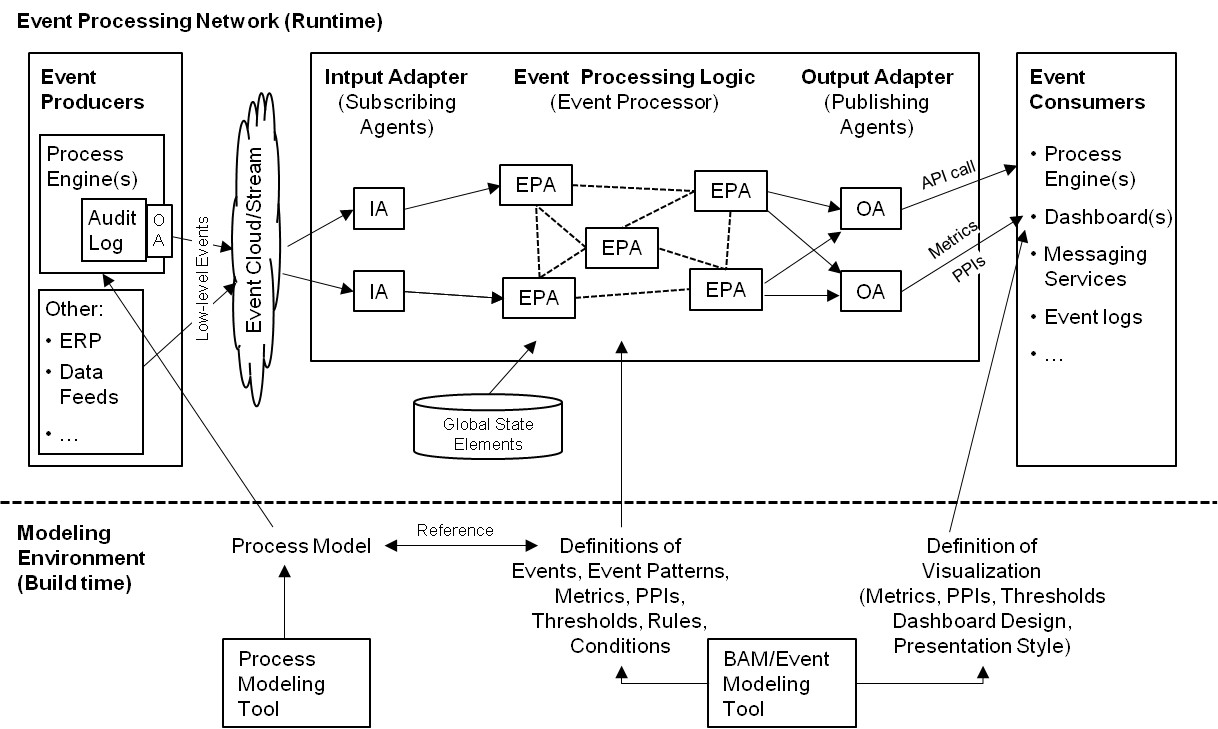
\includegraphics[width=0.9\linewidth]{Figures/Chapter5/Monitoring/Integrated-BAM-CEP-Architecture-27.jpg}
	\caption[Integrated BAM/CEP Architecture 27]{Integrated BAM/CEP Architecture \cite{book:processmonitoring}}
	\label{fig:BAMArchitecture}
\end{figure}



\subsection{Modeling BAM Parameters at Build Time}
As mentioned in the last section it is necessary not only to model the processes, but also numerous pieces of information relevant for a sound process monitoring in the sense of Business Activity Monitoring (BAM model). These can be derived from answers to questions like what, when, how and how often should be measured by whom \cite{book:ProzesseSchmelzer}. The information should also include how single metrics are to be aggregated in order to determine Process Performance Indicators (PPIs). For systematically collecting and documenting the necessary information fact sheets or templates for metrics and performance indicators have been developed \cite{book:KennzahlenIT}, \cite{book:ITControlling}. Figure \ref{tbl:Fact-Sheet}  shows an extract of a sample fact sheet defined for the average processing time of activities (see also \cite{article:SBPMCosting}, \cite{book:MonitoringSubjekt} ).


\begin{table}[htbp]
	\footnotesize
	\centering
	\begin{tabular}[t]{@{}l p{0.5\linewidth} p{0.3\linewidth} @{}}
		\toprule
		\textbf{Attribute} & \textbf{Content}  \\
		\midrule
		 & \textbf{Characteristics}
		\\
		Identifier & Average activity time
		\\
		Description & Average time of a process activity within a certain period
		\\
		To-be value/unit & tbd specifically (min.)
		\\
		Tolerance range/unit & tbd specifically (\%)
		\\
		Escalation Rules/ Actions & In case of violation alert the process owner and start escalation process (tbd specifically)
		\\
		Addressees & Process Owner, Middle Mangement, Accountants (tbd specifically)
		Responsibility	Process Owner (tbd specifically)
		\\
		&  &
		\\
		& \textbf{Measuring and Computing}
		\\
		Measuring Object & All instances of the process 'Purchase Order'
		\\
		(Single) Metrics & Start time and end time of all activities of the process
		\\
		Measuring Method & Read time stamps for beginning and end of activities written by Metasonic Flow 
		\\
		Measuring Frequency & For every single instance as it occurs
		\\
		Algorithms & For computing period: Sum of processing time of all activities divided by number of instances

		\\
		Data Sources (general) & Tables in the database of Metasonic Suite:
		RT\_PROCDESC, RT\_PROCINST, REC\_PARADESC, REC\_RECTRANS, UM\_USER
		\\
		Data Sources (specific) & Activity processing time (for one instance):\newline
		\textbf{SELECT} TIMESTAMP1  \newline
		(\textbf{SELECT} STARTTIME \newline
		\textbf{FROM} RT\_PROCINST \newline
		\textbf{WHERE} RT\_PROCDESC = \textit{process (purchase order)}\newline
		\textbf{AND} ID = \textit{instance (9)}\newline
		\textbf{FROM} REC\_RECTRANS\newline
		\textbf{WHERE} RT\_STDESC = \textit{\textit{state (fill\_in\_form)}}\newline
		\textbf{AND} RT\_PROCINST = \textit{instance (9)}
		Completed instances: see separate fact sheet .
		\\
		Computing Period (time, no. of inst.) & Daily
		\\
		& &
		\\
		& \textbf{Presentation}
		\\
		Presentation Style & As-is value and to-be value in combination with a spark line showing the historical development, deviation from to-be value in \%
		\\
		Presentation Frequency & Weekly and in case of escalation
		\\
		Archiving & Stored in additional database table, linked with RT\_PROCDESC
		\\
		
\bottomrule
\end{tabular}
\caption{Fact Sheet for a PPI (extract)}
\label{tbl:Fact-Sheet}
\end{table}

Replacing the content column by more formal ontology-based linguistic patterns as suggested by Del-Río-Ortega et al. (see table \ref{tbl:Fact-Sheet-PPI}) could help relating PPIs to elements of the process model, performing automated analysis \cite{article:ProcessPerfInd} and implementing the measurement at runtime. 

\begin{table}[htbp]
	\footnotesize
	\centering
	\begin{tabular}[t]{@{}l p{0.3\linewidth} p{0.4\linewidth} p{0.5\linewidth} @{}}
		\toprule
		\textbf{Attribute} & \textbf{Linguistic Pattern}  & \textbf{Example}\\
		\midrule
		PPI-<ID> & <PPI descriptive name> & PPI-001 Average time of RFC analysis
		\\
		Process	& <process ID the PPI is related to> & Request for change (RFC)
		\\
		Goals & <strategic or operational goals the PPI is related to> & BG-002: Improve customer satisfaction \newline
		BG-014: Reduce RFC time to response
		\\
		Definition & The PPI is defined as { \newline
			<DurationMeasure> | <CountMeasure> | <ConditionMeasure> |
			<DataMeasure> | <DerivedMeasure> | <AggregatedMeasure> }
		[expressed in <unit of measure>] & The PPI is defined as the average of Duration of Analyse RFC activity
		\\
		Target & The PPI value must { \newline
			be {greater | lower} than [or equal to] <bound> | \newline
			be between <lower bound> and <upper bound> [inclusive] |\newline
			fulfil the following constraint: <target constraint> } & The PPI value must be slower than or equal to 1 working day
		\\
		Scope & The process instances considered for this PPI are {
			the last <n> ones |
			those in the analysis period <AP-x> } & The process instances considered for this PPI are the last 100 ones
		\\
		Source & <source from which the PPI measure can be obtained> &	Event logs of BPMS
		\\
		Responsible & { <role> | <department> | <organization> | <person> } &	Planning and quality manager
		\\
		Informed &{ <role> | <department> | <organization> | <person> } & CIO
		\\
		Comments & <additional comments about the PPI> & Most RFCs are created after 12:00
		\\
\bottomrule
\end{tabular}
\caption{PPI Template based on Linguistic Patterns \cite{article:ProcessPerfInd}}
\label{tbl:Fact-Sheet-PPI}
\end{table}


Friedenstab et al. argue that such linguistic patterns do not fit to the usually graphical modeling of processes which makes integration difficult \cite{article:BPMNActivityMon}. The authors discuss some more approaches to BAM modeling. With regard to the limitations revealed, they present a BAM-related extension of the graphical Business Process Model & Notation (BPMN) \cite{article:BPMNActivityMon}.
Using an abstract language syntax based on the Unified Modeling Language (UML) they started defining meta models for language constructs needed for BAM as there are Duration, Frequency, Composed Basic Measure, Aggregated Measure, Filter, Target Definition, Actions, Measure-based Expressions and Dashboard. Figure \ref{fig:Meta-Model} depicts the example for the duration of elements on different levels of detail, where the grey colored parts indicate references to the BPMN specification.

\begin{figure}[h]
	\centering
	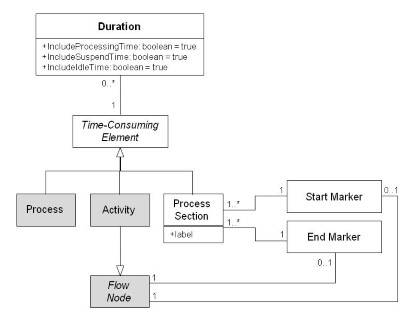
\includegraphics[width=0.9\linewidth]{Figures/Chapter5/Monitoring/Meta-Mode-fo-Duration-relate-to-BPMN-1.jpg}
	\caption[Meta Model for Duration (related to BPMN) 12]{Meta Model for Duration (related to BPMN) \cite{article:BPMNActivityMon}}
	\label{fig:Meta-Model}
\end{figure}


In a second step Friedenstab et al. developed a concrete syntax allowing for modeling the abstract language elements with graphical symbols and text labels. Parts of it are visible in figure \ref{fig:Model-Cycle-Times}. The example shows the BAM model for determining the cycle times of a purchase order process modeled in BPMN (lower part). The upmost part for example expresses the fact that the overall cycle time (Duration) for the last 50 instances (Filter) has to be determined and displayed on the dashboard (Dashboard). Monitoring the average of the overall cycle time for completed instances controls the modeled business logic of the process. If it is above 48 hours goods are delivered with an express shipping if the average cycle time is more than. Otherwise standard shipping is carried out. A deviation also leads to an alert sent to the process owner, while in any case the average is to be presented on the dashboard. The latter is also valid for the third time-related metric in the example, the partial cycle-time for the company-internal part of the process, which is set into relation with the overall cycle time.

\begin{figure}[h]
	\centering
	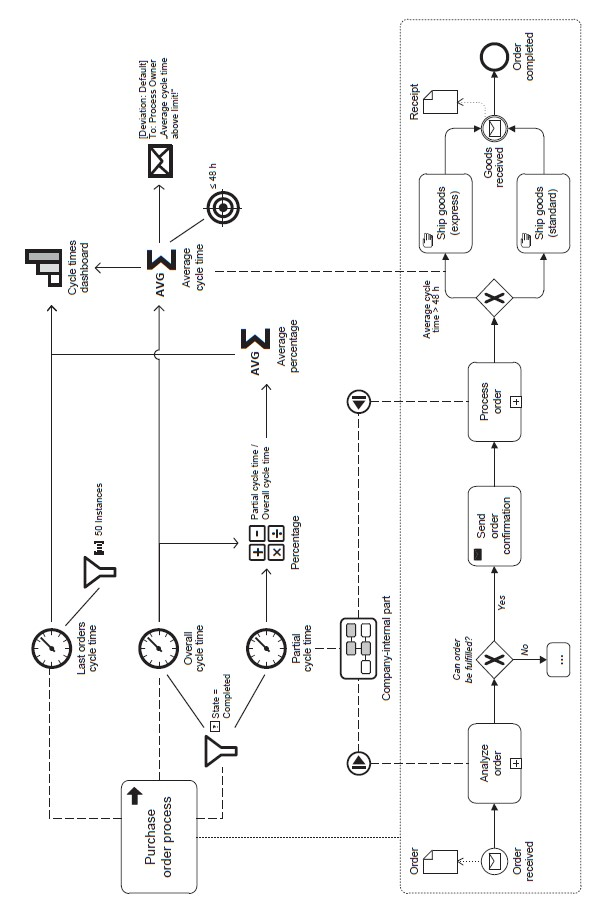
\includegraphics[width=0.9\linewidth]{Figures/Chapter5/Monitoring/BAM Model for Cycle Times.jpg}
	\caption[BAM Model for Cycle Times of a Purchase Order Process based on BPMN 12]{BAM Model for Cycle Times of a Purchase Order Process based on BPMN \cite{article:BPMNActivityMon}}
	\label{fig:Model-Cycle-Times}
\end{figure}


The concept presented by Friedenstab et al. is thoroughly thought-out and clearly and precisely elaborated. The idea now is to adapt it to Subject-oriented Business Process Management and relate the abstract syntax to the S-BPM meta model instead of BPMN. Due to S-BPM being a more precise and comprehensive notation than BPMN \cite{article:BPMNYAWLPatterns} the mapping should be possible without problems. Table \ref{tbl:MonBPMNSBPM} compares the BPMN specification elements used by \cite{article:BPMNActivityMon} with the ones appropriate in S-BPM \cite{Flei12}.


\begin{table}[htbp]
	\footnotesize
	\centering
	\begin{tabular}[t]{@{}l p{0.3\linewidth} p{0.4\linewidth} p{0.5\linewidth} @{}}
	\toprule
	\textbf{BAM Language Syntax Construct} & \textbf{Used BPMN Specification Element}  & \textbf{Suitable S-BPM Specification Element}\\
	\midrule\\
	Duration (Time-Consuming Element) &	Process, Activity, Flow Nodes&	Process, Subject Behaviour States (Function, Send, Receive, Start, End)
	\\
	Frequency
	(Countable Element)&	Process, Activity, Data Objects, Data States &	Process, Subject Behaviour States (Function, Send, Receive), Business Objects and their States 
	\\
	Actions &	Process	 & Process
	\\
	Measure-based Expressions &	Expression, Sequence Flow &	Incoming Message
	\\
	\bottomrule
\end{tabular}
\caption{BPMN and S-BPM Specifications used in BAM Constructs}
\label{tbl:MonBPMNSBPM}
\end{table}

The remaining constructs as well as the extensions do not depend on the process modeling language and thus are not included in the table.
On the other hand S-BPM, following its paradigm of regarding subjects, predicates and objects as equally important parts of a process, offers the subject as an additional specification element to add . In figure \ref{fig:Meta-Model-S_BPM} we modified the picture of figure \ref{fig:Meta-Model} by replacing the BPMN by S-BPM elements and adding the subject. This allows modeling the determination of the overall time a subject (respectively the allocated resource(s)) spends on working on a process instance. This is of interest for cost-related analysis.

\begin{figure}[h]
	\centering
	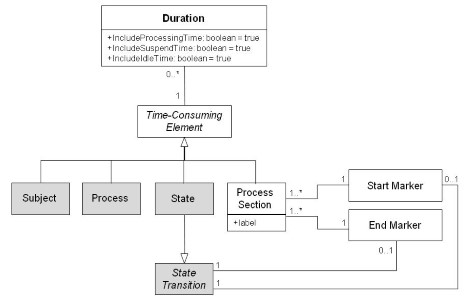
\includegraphics[width=0.9\linewidth]{Figures/Chapter5/Monitoring/Meta-Mode-fo-Duration-relate- to-SBPM.jpg}
	\caption[Meta Model for Duration (related to S-BPM)]{Meta Model for Duration (related to S-BPM)}
	\label{fig:Meta-Model-S_BPM}
\end{figure}


In order to show how the BAM language syntax constructs can be related to subject-oriented models we designed the purchase order process in S-BPM. Due to missing information in the BPM model some assumptions were necessary like who performs the process steps (subjects). We then added the BAM modeling symbols to create a monitoring model similar to that in figure \ref{fig:Meta-Model-S_BPM}.
The result is depicted in the following graph. In the lower part it includes the subject interaction diagram (SID) of the process. The SID shows the subjects involved and how they coordinate themselves in the course of action by exchanging messages. In the monitoring model in the upper part a difference can be seen. The partial cycle time for the company-internal activities can be modeled by just relating the clock symbol to the subject "Sales". In the example this subject represents all steps carried out within the organization. In the same way we can determine the cycle time for the other subjects.

\begin{figure}[h]
	\centering
	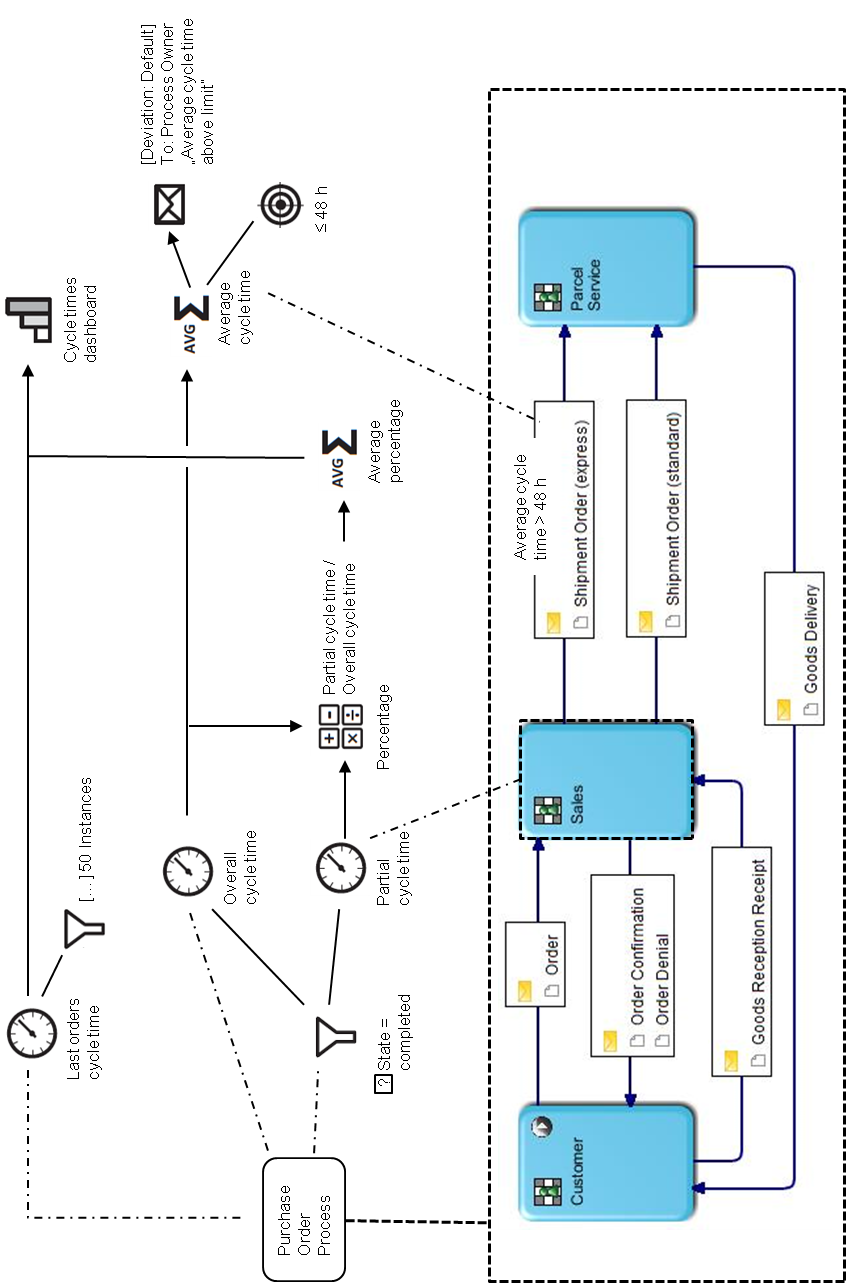
\includegraphics[width=0.9\linewidth]{Figures/Chapter5/Monitoring/BAM-Model-fo- Cycle-Times-of-a-Purchase-Order-Process-based-on-S-BPM.png}
	\caption[BAM Model for Cycle Times of a Purchase Order Process based on S-BPM]{BAM Model for Cycle Times of a Purchase Order Process based on S-BPM}
	\label{fig:Cycle-Time-SBPM}
\end{figure}

Given a special information demand a more granular modeling of BAM parameters is possible on the subject behavior level. Figure \ref{fig:BAM-Cycle-Time} for example details the behavior of "Sales" including all receive, send and functional states walked through by the subject. The symbols indicate that the average cycle time between order reception and confirming the order to the customer should be measured. In the same way cycle times between states in behaviours of different subjects can be modelled.


\begin{figure}[h]
	\centering
	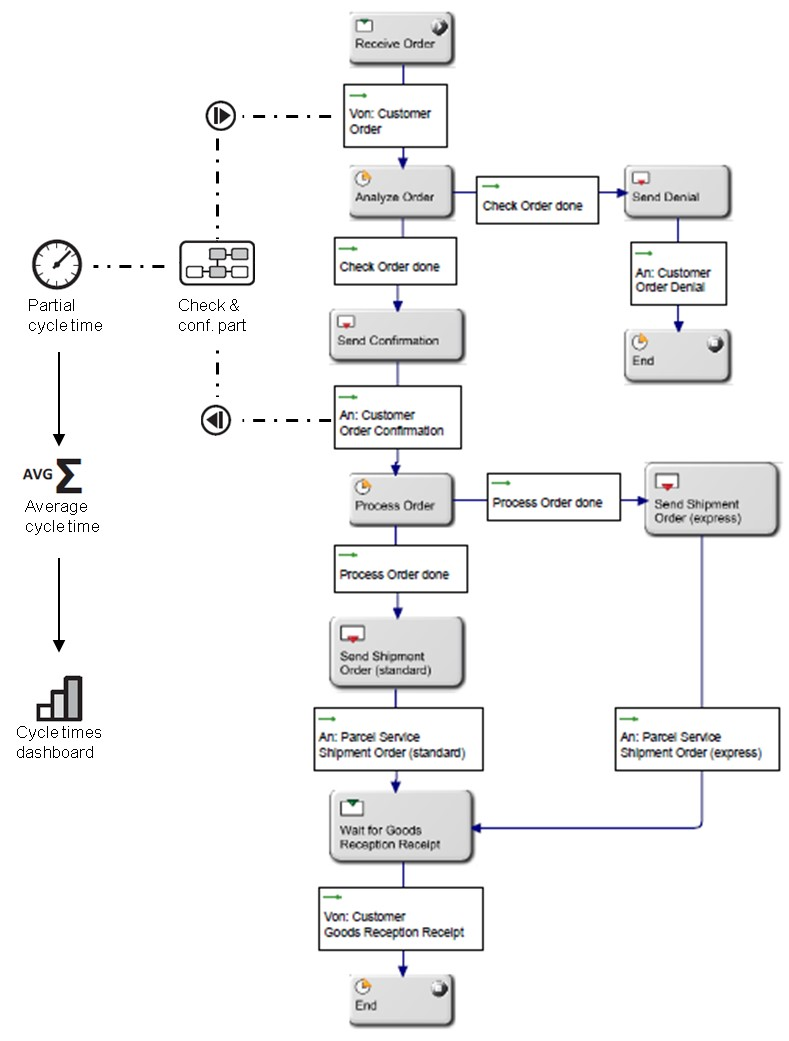
\includegraphics[width=0.9\linewidth]{Figures/Chapter5/Monitoring/BAM-Model-for-Cycle-Time-of-a-Process-Section-based-on-S-BPM.jpg}
	\caption[BAM Model for Cycle Time of a Process Section based on S-BPM]{BAM Model for Cycle Time of a Process Section based on S-BPM}
	\label{fig:BAM-Cycle-Time}
\end{figure}

Back on the level of subject interaction diagram we could also model to determine the overall time for receiving (waiting), sending and doing, both by process and by subject. Modeling on the two diagram levels reduces complexity.

\subsection {Conclusion and future Work}
This contribution systematized Business Process Monitoring and shed some light on the current state of monitoring in the context of S-BPM. Starting there we emphasized Business Activity Monitoring and took a closer look to the modelling of BAM parameters. We showed that the approach for BPMN presented by Friedenstab et al. can be adapted to S-BPM with little effort and that S-BPM shows additional potential to further develop the concept.
This is where future work needs to continue. The first step to go should be elaborating, detailing and tailoring the modeling language for the needs of S-BPM in order define a comprehensive basis for the succeeding task of developing easy-to-use software tool support. 
\\
The BAM modeling tool should make use of the model data created by the process modeling tool and add its results to a combined model base both for process execution and BAM. The third step would then be to build BAM functionality which at runtime processes events according to the subject-oriented BAM models. There is some evidence that S-BPM provides good premises to support event processing \cite{article:nondeterministicEvents}, e.g. by integration of a CEP Engine or single Event Processing Agents as subjects into processes. This has to be proven by a thorough investigation of the interrelationship and integration potential of CEP and S-BPM concepts and solutions. Generating code for BAM functionality out of the BAM model is another challenge to tackle \cite{article:BPMNActivityMon}. With the clear formal semantic of its underlying process algebra the S-BPM modeling language allows this for process models \cite{Flei12}. Consequently it seems to be worthwhile to investigate the possibilities of code generation out of BAM models too. 
\\
\\

\section{Subject Oriented Project Management}

In our global economy enterprises cooperate around the globe in order to create services or manufacture products for customers which are also distributed all over the world. The challenge of the cooperating partners as a federation of independent systems (virtual enterprise, VE) is to establish smooth cross-enterprise communication to reach the common objectives [1]. Information and communication technologies (ICT) are essential to create a federation of independent software systems suitable to execute business processes across the involved companies. 
\\
Figure 1 shows an example of an order-to-cash scenario where federated applications support a cross-company business process. A dog food store sells its products via internet. It commissions a transportation service provider to deliver the ordered products to the customer, who confirms the reception of the goods. The store deducts the money from the customer’s bank account. The process steps are facilitated by several independent software applications and message exchanges (order, order confirmation, delivery notification etc.) enabled by respective communication systems.
\\
Figure 1: Order-to-cash scenario in a federation of enterprises and applications (simplified)
Developing such a mutually adjusted solution by a federation of independent enterprises requires an approach different from traditional software development projects taking a process perspective (cf. [2]). Therefore our focus is on how to implement loosely coupled systems for exchanging information between independent partners, rather than tightly coupled solutions for sharing information or other resources.
The article is structured as follows. In section II we first take a look at virtual enterprises, federations of enterprise information systems, and their peculiarities, as they form the conceptual background of the proposal. Then, software development methodology and its elements are reviewed with respect to developing federated systems. This leads to section III, containing our proposal of a software development approach for federated systems based on subject orientation. We conclude in section IV.
\\
II.	BACKGROUND
A.	Recommendations for creating federated systems
When independent enterprises develop a federated system a lot of managerial and technological aspects have to be considered, particularly with respect to managing collaborative business processes. This is reflected in the following recommendations (cf. [3], [4]):
1.	Start the foundation of a federation and identify members.
2.	Identify and describe the business services that organizations can provide or they need from partners in service level agreements.
3.	Harmonize the enactment of collaboration by coordinating the participating organizations according to defined business processes and identify the systems required for the federation.
4.	Integrate the identified and implemented services/systems into the intended application. 
5.	Maximize the autonomy of organizations when collaborating, thereby ensuring organizations to benefit most from their own business objectives.
6.	Represent the partnerships between collaborating organizations when collaborating, and update changes in partnership.
7.	Guarantee the business privacy of organizations in the course of collaboration.
8.	Allow partners and other third parties to monitor, measure, and oversee the execution of business processes.
\\
B.	Federation of enterprise information systems
[1] define virtual enterprises and federations of enterprise information systems as follows: “The Enterprise partners’ Virtual Enterprise (EP VE) is the federation of partners in the community that come together to achieve the goal of a federated distributed system environment, sharing their resources, and collaborating to achieve a common goal: the Federated System VE (FS VE). The partners in the federation retain autonomy over their resources, deciding which resources (personnel, resource dollars, equipment, etc.) are sharable for achieving this goal. The results of this VE are then useable by the partners in furthering their individual systems. The FS VE is seen to be a virtual system of distributed processing components (hardware and software), which are physically implemented and managed by the partners. It is a federation of the partners’ systems, where each system retains its autonomy over all processing system components and sharable data/information. Retaining autonomy means defining which data or information and software/hardware assets will participate in the federation and be accessible and usable by other systems in the federation.”
The definition shows that the focus is on sharable resources. This means when setting up a federation the VE members need to clarify ownership of the shared resources as well as access rights and the rights to change those. Such an approach often implies tight coupling of the involved enterprises and the related resources. Entities leaving a federation then cause difficulties with respect to separating involved systems (changing access rights) and sorting out ownership of information.
Alternatively, information can be exchanged between the partners by messages, implying only a loose coupling of the involved systems. In this case the partners only need to agree upon structure and meaning of the data, e.g., using XML schemes, and upon the implementation of the message exchange, e.g., by web services. 
\\
C.	Software development methodology
“A software development methodology is a collection of procedures, techniques, tools and documentation aids which help developers to implement software systems” [5]. It may include modeling concepts, tools for model-driven architecture, integrated development environments (IDEs) etc. The so-called magic triangle (see figure 2) summarizes the various aspects of a software development methodology [6].

Figure 2: Magic triangle of software development methodologies
Concepts and Techniques are used to create models of the software to be implemented, and are thus significantly influencing which languages, procedures and tools are utilized. The applied concept implies the artifacts to be produced, of which the executable software system is the most important one. The Language is used to create the artifacts and tools. Procedures describe the sequence in which the activities for creating the various artifacts are executed. While languages and tools can be replaced without impacting concepts and procedures, the latter are decisively determining the shape of a software development environment.
\\
D.	Modeling concepts
Developing a federated system like the one described in section I requires modeling cross-company business processes and the entities performing activities in these processes.
1)	Business process modeling
There are various approaches for specifying business process models. IT implementations of those models are called process-controlled applications [7] or workflows. The modeling approaches can be distinguished in three classes: (i) Control flow-based specifications put the focus on the activities. (ii) Object-based models mainly describe business objects and the sequence of operations to manipulate them. (iii) Communication-based models focus on the active entities in a process which exchange messages in order to coordinate their work.
By their nature the latter are promising candidates for modeling federations of systems. Business Process Model and Notation (BPMN), the currently most widely discussed modeling language, contains elements for the description of control flows and communication in business processes. In the following we discuss its communication-oriented features.
To model communication BPMN provides so-called pools, each representing a process that can exchange messages with processes in other pools. Conversation diagrams are the means to describe this mechanism: However, they do not allow specifying the sequence in which messages are exchanged. Although the sequence can be captured by collaboration diagrams, the semantics of sending and receiving messages is not precisely defined. For instance, it remains unclear whether messages are exchanged synchronously or asynchronously. Additionally a certain message from a pool can only be received in a single activity state, but not in other states. Choreography diagrams in BPMN also define the allowed message sequence between pools. [8] describe a choreography-based tool for specifying global processes. The problem is that choreography specifications cannot contain data. As a consequence a modeler can only describe message sequences being covered by regular expressions, which is the lowest level in the Chomsky hierarchy. This fact makes it impossible to model a behavior like the following: Pool S sends n messages of a type X to pool R. After that S sends a message Y to R. Subsequently S expects m messages of type A from pool R, which received the n messages of type X. The reason for that is that the messages cannot be counted, because data are not allowed in BPMN choreographies.
Given these properties of BPMN this notation has significant draw backs for modeling communication, hindering the precise development of federations of systems.
2)	Multi-agent systems modeling
The term agent has multiple meanings. We follow the definition given in [9]: An agent is an entity that performs a specific activity in an environment of which it is aware and that can respond to changes. A multi-agent system (MAS) is a system where several, perhaps all, of the connected entities are agents. The most important property of agents is their controlled autonomy: They independently execute their role-specific behavior, and in multi-agent systems they communicate with each other. These properties are alike those of federated systems which therefore can be considered as multi-agent systems. This means that software development methodologies for agent-oriented software (for an overview see [8]) can help developing federations of applications.
\\
E.	Procedures
Software Life Cycles (SLC) build a framework for software development procedures. All software development projects follow a series of phases. While software life cycles can be defined in many different ways, each of them comprises the following generic activities:
•	Project conception or initiation
•	Planning
•	Execution with specification and implementation activities
•	Termination
In the traditional waterfall approach these activities are performed in the sequence shown above. Other life cycle concepts propose overlapping the development steps, suggest alternatives like the V model or agile development procedures like Extreme Programming and Scrum. [10], [6] and [5] give an overview of the various approaches.
\\
F.	Work break down structure (WBS)
The work break-down structure describes the work to be done in a project in a hierarchical way. A work break-down structure element may be a product, data, service, or activity contained in the software life cycle or any combination thereof. A WBS also provides the necessary framework for detailed cost estimating and control along with guidance for schedule development and control. The top level of the WBS should identify the major phases and milestones of the project in a summative fashion. Consequently, the phases used in the top level depend on the software development methodology applied in a project. The first level can either represent the phases used in the software life cycle or the major artifacts of the system to be developed. In case the top level is SLC-oriented it might be built by requirement specification, software architecture, programming, test etc. In the case of an evolutionary life cycle there will be topics like Release 1, Release 2 etc., followed by headlines like requirement specification on the second level.
Another alternative is to use top level headlines corresponding to artifacts created by modeling activities, such as ‘create communication structure’ or ‘describe subject behavior’ (see section III.D).
The WBS is created during the planning phase of a project life cycle. During this phase the project manager works with the project team to make sure that the client's needs are addressed and the project is planned completely and approved by the client prior to any sort of production beginning on the project.
G.	Organisational break down structure and software architecture
An organizational breakdown structure (OBS) complements the WBS and resource breakdown structure of a project. Project organizations can be broken down in much the same way as the work or product. The OBS is created to reflect the strategy for managing the various aspects of the project and shows the hierarchical breakdown of the management structure. Hence, the work break down structure has a significant impact on the organizational structure of the project team. The same holds for the phases of the software life cycle and the system architecture influencing the work break down structure. Conway’s law states “organizations which design systems ... are constrained to produce designs which are copies of the communication structures of these organizations” [11]. A variation of Conway’s law can be found in [12]. "If the parts of an organization (e.g., teams, departments, or subdivisions) do not closely reflect the essential parts of the product, or if the relationship between organizations do not reflect the relationships between product parts, then the project will be in trouble... Therefore: Make sure the organization is compatible with the product architecture” [12].
As we look at developing federations of systems with a federation of independent project teams, the system architecture needs to be aligned with the multiple project team structure.
\\

III.	SOFTWARE DEVELOPMENT METHODOLOGY FOR FEDERATED SYSTEMS
The software development methodology for federated systems proposed here is based on Subject-oriented Business Process Management (S-BPM) as the most straightforward enabler of communication-oriented BPM [16]. Therefore we first outline this approach the way being used in many industrial projects successfully (for examples see [13], [14], [15]). We then explain all activities and steps of the development cycle for describing and implementing a federated system using the dog food order-to-cash example. The sample case starts with having the idea to create a solution and ends with a running application.
\\
A.	Subject-oriented business process models
1)	Subjects, messages, and business objects
Subject-oriented business process management includes a modeling language for describing processes as a system of independent entities which organize their work by exchanging messages. Each entity is autonomous in the sense that it decides by itself when it sends messages, receives messages and executes internal actions. These entities are called subjects and can be interpreted as roles in a process to be implemented. Each subject has its local data which can be changed by local actions or by receiving messages. These data are called the business objects of a subject. Each message has a name, similar to a name of a method in object-oriented systems, and related business objects, which are send or received with it. If a message is sent it transmits the values of the business object. If a subject accepts a message by picking it up from the input pool (see section III.A.3), the values of the incoming business object are copied into a corresponding local business object of the receiving subject.
Physical things like a can of dog food can also be a business object. In general physical business objects are accompanied by data-oriented ones like a delivery slip. Consequently, a can of dog food together with the data of a delivery slip may form a combined business object. In the model data and physical entities are considered in the same logical way. The physical aspect of a business object is considered as implementation aspect. Such an understanding allows creating a model on a logical level independent from implementation details. These are added later on.
The sequence in which messages are sent, received, or internal actions are executed, is defined by the subject behavior (for details see section II.A.4).
2)	Subjects and agents
In order to execute subjects they will be assigned to agents or actors. An agent in that context is a human or non-human entity which is capable to execute actions. Details about the relationship between subjects and agents/actors can be found in [16]. This distinction allows to specify a federated system independent from a special environment. The subjects represent the members of a federation, and subjects can be assigned to another agent once the business relationship changes. Subject-oriented models are therefore independent from special members of a federation. For details about the deployment of subjects see [16] and [17] .
3)	Communication structure and message exchange
A communication structure shows which subjects are involved in a process and which messages they exchange. Figure 3 depicts the communication structure of the dog food order-to-cash application in the so-called subject interaction diagram (SID). It describes the system on a logical layer. What it does not show, is sending the message “deliver dog food” that is implemented by a truck transporting dog food cans together with a delivery slip. As we will see later on the exchange of all other messages are implemented using information and communication technology, and thus considered as aspects only relevant for implementation, but not for modeling (i.e. designing).

Figure 3: Communication structure of dog food order-to-cash application
The specification of the communication structure includes the business objects of each subject. It also defines which business object values are transported by which messages. The maximum number of messages which can be deposited in an input pool determines its size, independent on the size of the business objects coming with a message. In case the size limit is reached sending will be blocked until the receiving subject removes a message from its input pool. Alternatively, the incoming message replaces the most recent or message received initially in the pool, according to the chosen strategy. Details about message transfer and the related synchronization mechanisms are explained in [17].
A subject can receive certain messages by checking the input pool on their availability and removing those it finds. On removal the values of the transmitted business object are copied into a local business object. 
Figure 4 depicts the input pools of the subjects in our example. Since each subject sends one message to other subjects and then waits for an answer, all input pools have a maximum size of one.

Figure 4: Message exchange via input pools
4)	Subject behavior
Each subject executes send, receive and internal operations in a certain sequence. The allowed sequence is defined in a subject behavior diagram (SBD). Figure 5 shows the SBD of the subject “dog food store”. In the start state “wait for…” the subject waits for the message “order” from subject “customer”. After that the message “get money” is sent to the subject “bank”. If the message “money” comes from the subject “bank” the message “order confirmation” is sent to the customer. Then, the internal operation “prepare order” is executed. 
This function includes activities like checking the availability of the ordered goods, preparing the dog food, and all accompanying documents for shipment and updating the inventory. If the goods are not on stock the customer gets an order confirmation indicating a delay. In case of availability the message “Transfer order” is sent to the subject “shipment company”. It contains data (delivery slip) and physical business objects (cans with food). According to the behavior specification the subject then waits until the delivery confirmation arrives from the shipment company and subsequently terminates processing the instance. 
\\
B.	Development as a multiple-team structure
We now assume that the dog food order-to-cash scenario does not yet exist. The store wants to extend its services for the customers by offering online shopping and home delivery. In order to reach this business objective it takes the initiative to found a federation of enterprises which combine their services and develop a corresponding federation of systems.
Each federated enterprise establishes a project team, working on their parts of the solution independent from each other. This leads to a multiple-team project on the federation level [18]. As the teams belong to different, independent companies they all have their own development culture and methodology.
Since there is no single line management who can assign an overall project manager, the federation members need to agree on a project leader and the competencies related to this role. As the initiator of a federation has the most interest in the development of the federated solution it might be helpful that this company, in our case the store, recruits the leader.


Figure 5: Behavior of the dog food store (clipped)

His or her major task is to ensure smooth communication between the independent teams, respectively their managers. The project teams needs to coordinate how the systems they are developing communicate with each other. Their major communication paths are predefined by the communication structure of the system federation. This strategy leads to a high socio-technical-congruence. Figure 6 shows the team and communication structure of the dog food order-to-cash federation.

Figure 6: Multiple-team project and its communication structure
Beside that top-level communication implied by the problem structure, each team can use services offered by other enterprises. Figure 6 reveals that the shipment company uses the service of carriers and forwarding agents, in order to implement the transportation service offered to the dog food shop. This communication relation is of no interest for other federation members and thus should not be visible to the top level teams. It belongs to the internal issues of the shipment project team.
\\
C.	Development process for federated systems
In section III.A. the method for defining the functional requirements of a federated system was outlined. The artifacts to be created according to the method need to be developed by the federation of teams.
1)	Specification of the communication structure
The communication between the various members of the federation needs to be specified in more detail. This is done by assigning a subject to each member of the federation and defining the messages exchanged between the subjects. Consequently, a first version of the communication structure as described in section III.A.3 emerges. Together with the data transported by the messages a communication model of the system federation is defined. The advantage of the subject-oriented approach is that the system communication structure is directly in line with the communication structure of the corresponding developing teams. The result of that step is the subject interaction diagram (SID) as shown in Figure 3. 
2)	Specification of the subject behaviour
After defining the communication structure the behavior of each subject is specified. The modelers describe the allowed sequence of messages exchanged on top level and the internal functions of the individual systems. These internal functions represent the services executed by the corresponding federation partner either directly or supported by other service providers. They also encapsulate the communication with those sub-contractors as it is of no interest on the top level of the federation.
The behavior of a subject is mainly defined by the corresponding project team, however, in close coordination with the teams responsible for the partner subjects. The teams only need to make sure a message sent to a partner has a receive state in the corresponding subject behavior and vice versa. This pairwise coupling means, e.g., that the behavior description of the shipment company has to contain a state for receiving the “Transfer order” message, transmitted by the related send state in the behavior diagram of the dog food store subject (see figure 5). In order to correctly model these interactions the responsible project teams need also to agree on the interaction sequence of the subjects. However, their internal task behavior (i.e. sequence of functions for task accomplishment) might not become visible to others, as is specified decentralized and might not be shared at all. 
3)	Implementation of the input pool
The input pool is the abstract concept for defining the semantics of message exchange. Partners exchanging messages need to agree on how they implement the input pool semantics. Sending requires the sending subject to execute a function to deposit a message in the input pool of the receiver. For each subject doing so an implementation agreement is necessary. Since an input pool is owned by exactly one subject, the functionality for accessing it is local and does not need to be coordinated with the partners. In most cases input pools are implemented as web services.
4)	Implementation of subject behaviour
Each team has to implement the behavior of its subject. This means they have to ensure that depositing and removing messages (including business objects) in or from the input pool are executed and internal functions are invoked in the specified sequence. Workflow engines are appropriate tools for implementing that functionality.
5)	Implementation of internal functions
The internal functions realize the kernel of the service contributed by a partner to a federated application. Messages are the means to cause the invocation of an internal function, and they transport its result to a partner subject. Internal functions can be based on existing systems, e.g., an SAP client.  They also can be implemented using another federated solution, or being developed from scratch. The way an internal function is realized is a local decision taken by the corresponding project team.
6)	Operation of a federated system
Beside the development and deployment the non-functional aspects of a federated system need to be agreed upon by the contributing partners. For this purpose they negotiate service level agreements (SLA) defining response time, down time, reaction time in error cases etc. The SLA also includes business aspects like costs and regulations for exceptional situations like a member leaving the federation and bringing in another one.
D.	Federated work break down structure
The various activities described so far can be organized in a federated work break-down structure as shown in figure 7.

Figure 7: Work break down structure for the development of a federated system 
The tasks can be divided into three types:
Joint work concerns the top level of the federation and therefore is done collaboratively by all members of a federation. The major issue on this level is to agree on communication structure and behavior of the entire system, while the behavior of each subject can be described individually by the corresponding member of the federation.
Some work can be done bilateral. Communicating partners, e.g., agree on the coding of the business objects and the implementation of the input pool. They also define the service level agreements.
Local work comprises activities of the development teams which do need to be coordinated with teams of other federation members. A major example in this context is the set of internal functions of each subject, being a local matter, and developed following the particular culture and methodology of the respective team.
\\
E.	Continuous alignment by communication

Although development can be split in joint, bilateral and local tasks accomplishment continuous communication is essential for the sustainable success of the resulting federated system.
The overall project leader and the team managers need to swiftly exchange all relevant information in order to maintain the solution according to the changing requirements of the partners.
\\
F.	Validation

The described development methodology has been partially applied in several cross-organizational industry projects. The organizations belonged to the same enterprise, which allowed a central project management. Due to restrictive permission regulation of the industry partners the publication of experiences is not possible so far. Hence, we have set up a field study to deepen our practical experiences with the presented approach. 
The case deals with establishing novel services for co-housing activities, namely to support groups of people to design and implement a common housing project (see also www.tsibutsang.at, www.artsliving.at). For each housing project a project leader needs to be established, stemming either from the co-housing support provider or another project partner, e.g., a construction company. He/She ensures communication and coordination of parallel and distributed activities. For each project, various company procedures have to be aligned and a federated system has to be established. 
\\
1)	Specification of the communication structure
In a workshop, the communication between the various members of the federation is specified. This step is supported by holomapping (www.vernaallee.com), as it allows identifying functional roles in a straightforward way.  Once having determined them as set of holomap nodes, a subject can be assigned to each member of the federation – in the case of co-housing the cohousing service provider, the co-housing group (customer), architect (for planning), and an engineering company (for building). Moreover, the tangible relationships of holomaps represent deliverables and as such, messages exchanged between the subjects. These relationships also indicate the data transported by the messages, thus facilitating the specification of business objects, such as contracts that need to be set between the various co-housing parties.
\\
2)	Specification of the subject behaviour  
Each contributing co-housing project partner (subject) has a certain behavior that needs to be detailed not only in terms of exchanging messages (i.e. the communication structure) but in terms of concrete activities (internal functions). For instance, the co-housing provider needs to arrange rooms for meetings, schedule social activities and prepare for documenting results of negotiations. These activities are mainly executed by functions provided by the cohousing providers’ platform http://tsibutsang.mixxt.org/. In this case, mixxt is that federation partner’s service provider. The project leader needs to ensure the completion of behavior specifications, in particular when adaptations of standard procedures, such as contracting for taking over land before authority clearance, are required,. Upon completion, the co-housing project is operationalized in terms of complete send-receive interactions between all project parties. 
\\
3)	Implementation of the input pool
In that step project-specific semantics of message exchange is defined. For instance, , a message in the input pool of the co-housing support provider is based on the implementation agreement that each partner (engineering company, co-housing group) can send request messages  any time with a fixed max. response time of 2 workdays. Such an agreement is due to the eventuality of social conflicts that should be addressed promptly. 
\\
4)	Implementation of subject behaviour
Since in our field study workflow management systems are not being used, each involved organization needs to ensure the negotiated communication pattern with its partners. The co-housing support provider is using its mixxt-platform to trigger the (internal) project coordinator of the respective project. Hence, for each project, a dedicated workspace is established including a corresponding input pool thus enabling a dedicated communication pattern and set of business objects for each project.
\\
5)	Implementation of internal functions

Typical internal functions in the field study are requests triggering further communication or processing data by the addressed subject (project partner). For instance, a meeting of a co-housing group needs to be established, once all biddings for a certain completion step have arrived from the engineering company. Meetings are arranged invoking www.doodle.com  from the meeting space of the mixxt-platform.
\\
6)	Operation of a federated system
Typical non-functional aspects of a federated system in co-housing concern the agreement to set up a task force in case of unforeseen events, selecting relevant partners to resolve all issues related to these events. Other agreements concern costs and results from regulation checks influencing original co-housing plans. Finally, changing the federation’s structure in terms of membership and responsibilities is also regulated by dedicated agreements.

IV.	CONCLUSION AND FURTHER WORK
We have presented an approach for developing federated systems. The concept considers the characteristics of virtual enterprises combining the services of the partners to satisfy customer needs while keeping legal, organizational, technological and cultural independence.
Our communication-oriented view follows the idea that the decentralized structure of federated systems needs to be reflected in the organizational structure of multiple project teams for developing such systems. Those teams belong to separate enterprises and are mutually independent with respect to methodology, technology etc. they use to develop their individual part of the federated system. 
The proposed approach establishes a layer above the enterprise-specific environments. It helps building coherence on the top level of the federated system solution, while the teams, system elements etc. on the individual level of each federation member keep the highest degree of independence.
\\
REFERENCES
\\
[1] 	J. Putman and S. Strong, "A Federated Virtual Enterprise (VE) of Partners, Creating a Federated VE of Systems," IEEE Proceedings of Compsac, 1998. 
\\
[2] 	V. Gruhn, „Process-centered software engineering environments, a brief history and future challenges,“ Anals of Software Engineering, pp. 363-382, 14(1-4) 2002. 
\\
[3] 	H. F. P. Smith, Business process management—The third Wave, Meghan-Kiffer Press, 2003. 
\\
[4] 	L. Chengfei, L. Qing and Z. Xiahui, "Challenges and opportunities in collaborative business process management: Overview of recent advances and introduction to the special issue," Information Systems Frontiers, pp. 201-209, 11 2009. 
\\
[5] 	D. E. Avison and G. Fitzgerald, Information Systems Development: Methodologies, Techniques and Tools, New York, NY.: 3rd ed. McGraw-Hill, 2003. 
\\
[6] 	J. Ludewig und H. Lichter, Software Engineering, 3. Edition, Heidelberg: d-punkt Verlag, 2013. 
\\
[7] 	V. Stiehl, Prozessgesteuerte Anwendungen entwickeln und ausführen mit BPMN, Heidelberg: d-punkt Verlag, 2013. 
\\
[8] 	R. Cognini and et. al., "HawkEye: A tool for collaborative Business Process modelling and verification," in SAC’13, Coimbra, Portugal, 2013. 
\\
[9] 	L. S. Sterling and K. Taveter, The Art of Agent-Oriented Modeling, Cambridge, Massachusetts: The MIT Press, 2009. 
\\
[10] 	R. Ramsin and R. F. Paige, "Process-centered Review of Object Oriented Software Development Methodologies," ACM Computing Surveys, Vols. Volume-40, Number 1, 2008. 
\\
[11] 	M. E. Conway, "How do Committees Invent?," vol. 14, 1968.
\\ 
[12] 	J. O. Coplien and N. B. Harrison, Organizational Patterns of Agile Software Development, Prentice Hall International, 2004. 
\\
[13] 	T. Walke and et. al., "Case Study @ Swisscom (Schweiz) AG: iPhone 5 Self-Service Order App and Process-Workflows," in H. Fischer, J. Schneeberger (Ed.), S-BPM ONE - 2013, CCIS Vol. 360, Heidelberg, Springer Verlag, 2013. 
\\
[14] 	G. Konjack, „Case Study: AST Order Control Processing,“ in H. Buchwald et.al. (Eds.), S-BPM ONE - Setting the stage for Subject Oriented Process Management, CICS Vol. 85, Heidelberg, SPringer Verlag, 2010. 
\\
[15] 	S. Nakamura and e. al., "CGAA/EES at NEC Corporation, Powered by S-BPM: The Subject-Oriented BPM Development Technique Using Top-Down Approach," in W. Schmidt (Ed.), S-BPM ONE - Learning by Doing - Doing by Learning, CCIS Vol. 213,, Heidelberg, Springer Verlag, 2011. 
\\
[16] 	A. Fleischmann, U. Kannengiesser, W. Schmidt and C. Stary, "Subject-Oriented Modeling and Execution of Multi-Agent Business Processes," Atlanta, 2013. 
\\
[17] 	A. Fleischmann, W.Schmidt, C. Stary, S. Obermeier and E.Börger, Subject Oiented Business Process Management, Berlin, Heidelberg: Springer, 2012. 
\\
[18] 	R. K. Wysocki, Effective Project Management, Seventh Edition, Indianapolis: John Wileys & Sons, 2014. 
\\
[19] 	E. Yu und et. al., Social Modeling for Requirements Engineering, Cambridge, Massachusetts: The MIT Press, 2011. 





